\documentclass[12pt,a4paper]{article}
\usepackage{fullpage}
\usepackage{setspace}
\usepackage{parskip}
\usepackage{titlesec}
\usepackage[section]{placeins}
\usepackage{xcolor}
\usepackage{breakcites}
\usepackage{lineno}
\usepackage{hyphenat}
\usepackage{times}
\PassOptionsToPackage{hyphens}{url}
\usepackage[colorlinks = true,
            linkcolor = blue,
            urlcolor  = blue,
            citecolor = blue,
            anchorcolor = blue]{hyperref}
\usepackage{etoolbox}
\makeatletter

\makeatother
\usepackage{natbib}
\renewenvironment{abstract}
  {{\bfseries\noindent{\abstractname}\par\nobreak}\footnotesize}
  {\bigskip}
\titlespacing{\section}{0pt}{*3}{*1}
\titlespacing{\subsection}{0pt}{*2}{*0.5}
\titlespacing{\subsubsection}{0pt}{*1.5}{0pt}
\usepackage{authblk}
\usepackage{graphicx}
\usepackage[space]{grffile}
\usepackage{latexsym}
\usepackage{textcomp}
\usepackage{longtable}
\usepackage{tabulary}
\usepackage{booktabs,array,multirow}
\usepackage{amsfonts,amsmath,amssymb}
\providecommand\citet{\cite}
\providecommand\citep{\cite}
\providecommand\citealt{\cite}
% You can conditionalize code for latexml or normal latex using this.
\newif\iflatexml\latexmlfalse
\providecommand{\tightlist}{\setlength{\itemsep}{0pt}\setlength{\parskip}{0pt}}%
\AtBeginDocument{\DeclareGraphicsExtensions{.pdf,.PDF,.eps,.EPS,.png,.PNG,.tif,.TIF,.jpg,.JPG,.jpeg,.JPEG}}

\usepackage[utf8]{inputenc}
\usepackage[brazil]{babel}
\usepackage{float}
\iflatexml
\else
\fi


\begin{document}

\title{Análise da resistência à flexão e ao crateramento de uma~ engrenagem
cilíndrica de dentes retos: avaliação da eficácia da norma ANSI/AGMA~
2101-D04\selectlanguage{brazil}}

\author[1]{David Lira Nunez}%
\affil[1]{Federal University of Technology - Paraná (UTFPR)}%

\vspace{-1em}

\date{\today}

\begingroup
\let\center\flushleft
\let\endcenter\endflushleft
\maketitle
\endgroup

\selectlanguage{brazil}
\begin{abstract}
Um dos elementos de transmissão mais usados e que ainda proporciona a
inclusão de novas tecnologias na Engenharia Mecânica é a engrenagem de
aço cilíndrica de dentes retos. Embora seja um elemento mecânico muito
usado na indústria e testado pelos cientistas, há pouca informação
atualizada e disponível sobre seu equacionamento no Sistema
Internacional para o cálculo à fadiga: análise de tensão ao contato e
consequente avaliação da resistência ao crateramento na superfície do
dente da engrenagem; análise da tensão à flexão e consequente avaliação
da resistência a fratura na região do cordão raiz do dente da
engrenagem. Para tal, tem-se mapeado os artigos mais relevantes dos
últimos 8 anos da área de Engenharia Mecânica que abordam a análise
desse elemento mecânico, destacando a norma ANSI/AGMA 2101 para o
sistema internacional. Nesse sentido, o presente trabalho detalha dita
norma e a complementa com informações da literatura consolidada de
Projeto de Máquinas, proporcionando ao mundo acadêmico e industrial,
mais um material que possa auxiliar no projeto para a análise de uma
engrenagem, nos~ seus cálculos de análise à fadiga e mitigação de
possíveis falhas causadas por erros de projeto. Para maior entendimento
da aplicabilidade dessa norma, foi desenvolvido um estudo de caso que
compara a norma AGMA com resultados obtidos no software Solid Edge que
usa para seus cálculos a norma ISO 6336. O principal resultado deste
trabalho é a comprovação que os resultados de ambas normas diferem
muito, sendo os valores no Solid Edge mais conservadores. Finalmente,
este trabalho compartilha uma planilha com todo o equacionamento para a
análise analítica de qualquer engrenagem cilíndrica reta de aço,
seguindo a modelagem analítica da norma ANSI/AGMA.

\textbf{Palavras-chave:} AGMA 2101-D04. Engrenagem cilíndrica reta, ISO
6336. Solid Edge.%
\end{abstract}\selectlanguage{Brazil}%

\newpage

\sloppy

\selectlanguage{Brazil}\section*{Introdução}

{\label{introduuxe7uxe3o}}

Na grande área de Engenharia Mecânica, a engrenagem é um elemento mais
relevantes associado ao Projeto de Máquinas são, que transmitem rotação,
torque e potência entre eixos por meio do engate de dentes com involutas
especiais. Mudando os diâmetros desses elementos podem ser aumentadas as
velocidades de rotação de um eixo e diminuir o seu torque, manter a
velocidade e o torque constantes ou reduzir a velocidade de rotação e
aumentar o torque \hyperref[csl:1]{(Wicker \& Lewis, 2015)}.

A grande maioria de falhas que pode apresentar uma engrenagem tem origem
em anomalias associadas ao seu uso incorreto, tais como montagem e
lubrificação inadequadas, sobrecargas, etc. As falhas podem ser
classificadas em: desgaste, fratura por fadiga e deformação plástica.
Além disso, uma das principais causas que produz ditas falhas é devido a
erros no projeto e de fabricação \hyperref[csl:2]{(Amaral, 2012)}.

Nesse contexto,~\hyperref[csl:3]{(Lisle et al., 2017)}, consideram uma análise de tensão à
flexão de uma engrenagem cilíndrica de dentes retos pode ser obtida de
forma analítica por meio das normas ISO~\hyperref[csl:4]{(6336-3, 2006)} e
ANSI/AGMA~\hyperref[csl:5]{(2101-D04, 2016)}. Já para uma análise por simulação
computacional de elementos finitos (FEA do inglês~\emph{Finite Element
Analysis}) pode ser usado o software ANSYS, por outro lado, quando é
preciso realizar uma análise estática com testes experimentais, o uso do
extensômetro é apontada como a técnica mais usada.

Para testes experimentais, especificamente quando usado o extensômetro,
um fator que induzir a erros de coleta de dados é a posição inadequada
do extensômetro no cordão raiz do dente, e isso ocorre pelo tamanho do
filete que normalmente oferece um espaço limitado para a montagem do
sensor.

Por outro lado, ao usar a norma ISO ou AGMA existem discrepâncias quando
comparados seus resultados. A literatura aponta que isso deve-se
principalmente a como cada norma considera a geometria do dente da
engrenagem, especificamente o efeito no filete do cordão raiz. A ISO
considera uma parábola base com ponto tangente de um triângulo reto de
30°, já a norma AGMA considera a parábola de Lewis. Além disso, o cordão
raiz usando a norma ISO é praticamente o dobro daquele usando na norma
AGMA. Também, aponta-se que na norma ISO considera-se apenas a carga
tangencial, já na norma AGMA considera-se a carga tangencial e radial.
Finalmente, outro motivo de discrepância entre ambas normas deve-se ao
fator de concentração de tensão à fadiga, a norma AGMA é 9,3\% menor do
que a norma ISO, e por esse motivo a norma ISO pode ser considerada,
também, mais conservadora do que a norma AGMA,~\hyperref[csl:3]{(Lisle et al., 2017)}.

Na análise de uma engrenagem, usando o software ANSYS para FEA,
aponta-se que a melhor forma de estudar a engrenagem é com a
representação de apenas 3 dentes da engrenagem. Mas, embora destaca-se o
ANSYS na precisão de resultados, essa análise leva em consideração
apenas cenários de projetos limitados quando comparados a engrenagens em
funcionamentos reais que sim são consideradas nas normas AGMA e ISO.
Sendo assim, nesse estudo pode-se concluir que a modelagem analítica da
norma AGMA é mais real na sua representação de um cenário industrial e
mais fácil de ser adotada na análise à flexão de uma engrenagem
cilíndrica de dentes retos~\hyperref[csl:3]{(Lisle et al., 2017)}.

No trabalho de \hyperref[csl:6]{(Marques et al., 2017)}, é realizado um estudo sobre o
comportamento da distribuição de carga ao longo da face do dente de uma
engrenagem. Para tal, são analisadas engrenagens cilíndricas de dentes
retos e de dentes helicoidais, usando as normas ISO 6336-3 (2006) e
ANSI/AGMA 2101-D04 (2016), testes empíricos usando extensômetro e
programas de FEA.

Um dos resultados desse trabalho foi a comprovação que ambas
engrenagens, de dente reto e helicoidal, possuem a mesma rigidez no
engrenamento, mas, afirmam que os dentes helicoidais possuem um
engrenamento com variação mais gradual, o que consequentemente faz que
sejam mais suaves do que um de dentes retos. Além disso, nesse estudo
também comprovou-se que um dente quando possui alívio (remoção de
material), no adendo do dente da engrenagem, produz um engrenamento
ainda mais suave~\hyperref[csl:6]{(Marques et al., 2017)} .

Já no trabalho de \hyperref[csl:7]{(Wen et al., 2018)}, é analisado o cordão raiz do dente
de uma engrenagem cilíndrica reta, usando também as normas: ISO 6336-3
(2006), ANSI/AGMA 2102-D04 (2016), extensômetro e programas de FEA.
Nesse trabalho, destaca-se a facilidade e rapidez de análise do cordão
raiz de um dente de engrenagem usando ferramentas de FEA, já que pode
ser atualizada constantemente a geometria do elemento em estudo, sem
nenhum custo de insumo ou processo de fabricação.

No caso de analise por meio de testes experimentais, além de destacar o
uso do extensômetro, apontam o método fotoelástico como uma boa técnica
que pode auxiliar na corroboração ou comprovação da eficiência de
modelos analíticos e/ou de simulação ~\hyperref[csl:7]{(Wen et al., 2018)}. Por outro
lado, os autores apontam um ponto negativo no estudo de uma engrenagem
quando usados testes experimentais ou de FEA, o custo envolvido em
softwares de simulação, processadores de computadores e insumos para
testes experimentais. Além disso, o tempo de análise normalmente é maior
nestas duas formas de análise do que a modelagem analítica. Também nos
testes experimentais um ponto negativo é que para poder analisar a
engrenagem ela deve ser ampliada, na sua reprodução, para poder coletar
dados confiáveis.

Por outro lado, quando comparadas as normas ISO e AGMA, a primeira
destaca-se quando usada para análise de engrenagens de dentes
helicoidais. Mas, o principal ponto negativo da norma ISO é que no seu
cálculo considera-se apenas a carga tangencial, e nesse estudo
destaca-se também o uso da norma AGMA por ser menos conservadora e mais
fácil de ser usada do que a norma ISO. Nesse trabalho, uma informação
importante é que o cordão raiz é o produto do módulo vezes a constante
0,38. Além disso, nesse trabalho comprova-se que a maior número de
dentes, a tensão no cordão raiz diminui, e quando o módulo aumenta
também é menor a tensão no cordão raiz \hyperref[csl:7]{(Wen et al., 2018)}.

No trabalho de~\hyperref[csl:8]{(Wei et al., 2019)} é analisada a tensão ao contato num
dente de engrenagem com tratamento térmico por cementação, de uma
turbina eólica. Nesse artigo, constatou-se que o ponto mais crítico de
contato é o flanco do dente que coincide com o diâmetro primitivo. Para
dito estudo foi usado o software ABAQUS para FEA e um dos resultados foi
a comprovação que com um tratamento térmico aumenta a sua vida útil ao
crateramento. A cementação usada para esse estudo possuía uma espessura
de 2,2 mm, onde na superfície constatou-se uma dureza Brinell (HB do
inglês \emph{Brinell hardness}) de 620, a 1,5 mm de profundidade uma
dureza HB de 550 e a 2,2 mm a dureza HB foi de 400. Também afirma-se que
é na camada de 1,5 mm de profundidade que normalmente inicia-se a
fratura do dente quando submetido a mais de 10\textsuperscript{7}
ciclos.

No trabalho de~\hyperref[csl:9]{(Wen et al., 2019)}, analisam-se o efeito na tensão de
contato quando aplicado um alívio na ponta do adendo do dente da
engrenagem. Para esse estudo usou-se a FEA, métodos experimentais
(extensômetro), e cálculos analíticos baseados nas normas
ISO~\hyperref[csl:10]{(6336-2, 2006)} e ANSI/AGMA~\hyperref[csl:5]{(2101-D04, 2016)}. Destaca-se que
uma das maiores desvantagens encontradas nos seus estudos foi o tempo de
processamento e custo computacional, quando usado métodos de elementos
finitos (FEM -- do inglês \emph{finite Element Method} ),
especificamente quando a representação de malhas nas principais regiões
a serem analisadas numa engrenagem, (cordão raiz e flanco de contato).
Para os testes experimentais relata-se custos elevados com insumos e
materiais usados nas amostras e testes, além de não poderem reproduzir
fielmente toda uma engrenagem na sua escala natural (real). Dessa forma,
recomendam o uso de modelagem analítica baseados nas normas ISO ou AGMA.

Quanto aos principais modos de falha considerados numa engrenagem de
transmissão, a fratura no cordão raiz e o crateramento na superfície de
contato do dente são os mais frequentes e críticos, e é por esses
motivos que todos os estudos desse elemento de transmissão focam-se
nessas características geométricas. Assim, uma forma prática de diminuir
a tensão do cordão raiz é aumentando o número de dentes, e para diminuir
a tensão de contato é garantindo a qualidade do processo de fabricação,
oferecendo padrão no passo e forma geométrica de dentes, e no seu
acabamento superficial \hyperref[csl:11]{(Zhan et al., 2015)}.

Outras conclusões do trabalho de~\hyperref[csl:11]{(Zhan et al., 2015)} foram que para a análise usando testes experimentais, como o extensômetro, a engrenagem
precisa ser aumentada na sua escada de tamanho para poder ser analisada.
Para usar o FEM,a representação de apenas 3 dentes é indicada como
recomendada, dessa forma garante-se uma análise precisa e evita longos
processamentos computacionais. Já no uso de modelos analíticos
destaca-se a norma ANSI/AGMA 2101-D04 (2016), principalmente no uso da
análise de tensão ao contato. Nesse trabalho demonstrou-se que o alívio
na ponta do adendo do dente diminui a tensão de contato, mas ressalta-se
que se esse alívio não for calculado, (podendo ser grande demais), pode
aumentar a tensão de flexão no cordão raiz do dente, o que pode diminui
a vida útil do elemento.

No trabalho de~\hyperref[csl:12]{(Maper et al., 2019)} também realizam-se estudos na
inclusão de alívio na ponta do adendo. Nos testes realizados por esses
pesquisadores considera-se a criação de duas formas de remoção da ponta
do adendo: i) criar um chanfro na ponta do adendo, ou seja, uma remoção
linear de alivio, e ii) a criação de uma remoção côncava na ponta do
adendo. Para seus estudos foram usadas a norma ANSI/AGMA 2101-D04 (2016)
e o FEM com o software ANSYS, modelando apenas 3 dentes da engrenagem.

Um dos principais resultados constatados foi que para cargas
relativamente elevadas, o dente com alívio apresenta um engrenamento
mais suave quando comparado a um dente sem nenhum tipo de alívio na
ponta do adendo. Ambas remoções (linear e parabólica) diminuem,
aproximadamente, em 4,5\% a tensão ao contato e 2\% a tensão à flexão
~\hyperref[csl:12]{(Maper et al., 2019)}.

Em outros estudos usando a modelagem analítica das normas ISO 6336 e
ANSI/AGMA 2101, conclui-se, também, que a norma ISO é mais conservadora
e mais complexa no seu uso quando comparada com a norma AGMA
\hyperref[csl:13]{(Octrue et al., 2015)}.

Para um FEM, comprova-se também que uma boa análise é representando
apenas 3 dentes de uma engrenagem. E, considerando que em um par de
engrenagens o ângulo 0° é o início de rotação do engrenamento e, entre
2,7° a 27,4° de rotação da engrenagem é onde se apresentam as tensões de
contato, podendo concluir também que a 15° de rotação da engrenagem é
quando há maior contato no diâmetro primitivo. Além disso, demonstrou-se
que entre a coroa e o pinhão, o pinhão é a engrenagem que sofre maior
tensão de contato \hyperref[csl:14]{(Hwang et al., 2013)}.

No trabalho de \hyperref[csl:15]{(Geren \& Uzay, 2016)}, também destaca-se que uma das
principais causas de falha na indústria é a fratura no cordão raiz da
engrenagem. E para tal, afirma-se que a melhor forma de analisar uma
engrenagem cilíndrica de dentes retos é usando uma modelagem analítica
das normas ISO 6336 ou ANSI/AGMA 2101.

Podemos concluir que a modelagem analítica usando a norma
ANSI/AGMA~\hyperref[csl:5]{(2101-D04, 2016)} é a mais recomendada para reproduzir o
funcionamento real de uma engrenagem, além de ser mais fácil na sua
aplicação. E, podem ser feitas comparações dos seus resultados
analisados com FEM, destacando-se o software ANSYS, tendo uma grande
capacidade para FEA, mas, uma limitação é o tempo de modelagem 3D do
elemento. Para tal, o programa de modelagem 3D Solid Edge pode ser usado
para essa finalidade inicial, visto que já vem sendo usada para essa
função em alguns trabalhos relacionados à representação de
engrenagens~\hyperref[csl:16]{(Patil \& Kumar, 2017)}\hyperref[csl:17]{(Kumar \& Patil, 2017)}\hyperref[csl:18]{(Goanta \& Dumitrache, 2017)}\hyperref[csl:19]{(Pu et al., 2019)}.

Além disso, o programa Solid Edge possui uma plataforma que realiza o
cálculo analítico à flexão e ao contato para uma engrenagem cilíndrica
de dentes retos, usando a norma ISO 6336. Dessa forma, podem ser gerados
e comparados os resultados do Solid Edge com os do modelo analítico
usando a norma ANSI/AGMA 2101-D04 (2016). Porém, é muito importante
destacar que as publicações estudadas para este trabalho, consideram a
norma ISO 6336 versão 2006, para contato (parte 3) e para flexão (parte
2). Atualmente a norma ISO tanto para tensão à flexão e ao contato, de
uma engrenagem cilíndrica, já publicou uma nova versão em 2019, mas a
mesma não consta nas últimas pesquisas levantadas no estado da arte e
nem foi possível a sua aquisição para este trabalho.

No presente trabalho, será detalhada a norma
ANSI/AGMA~\hyperref[csl:5]{(2101-D04, 2016)} para uma modelagem analítica que analise a
resistência à flexão e ao crateramento de uma engrenagem cilíndrica de
dentes retos, seguido de um estudo de caso para posteriormente modelar
essa engrenagem no Solid Edge e realizar uma comparação crítica entre
ambos resultados. Futuros trabalhos pretendem realizar essa comparação
com o software ANSYS.

\section*{Fundamentação Teórica}

{\label{fundamentauxe7uxe3o-teuxf3rica}}

Neste capítulo é feito o detalhamento da norma AGMA \hyperref[csl:5]{(2101-D04, 2016)}.
Nesse sentido, entende-se que todo o material contido nesse capitulo é
usando dita norma como referencial bibliográfico, fato pelo qual não há
necessidade de citações constantes ao longo das próximas páginas deste
trabalho. Quando houver algum aporte no detalhamento da modelagem
analítica da norma AGMA, que sirva de complementação, tais materiais
serão citadas.

\subsection*{Resistência ao
Crateramento}

{\label{resistuxeancia-ao-crateramento}}

O objetivo da resistência ao crateramento é avaliar a vida útil da
superfície do flanco de um dente de uma engrenagem, frente ao desgaste
progressivo que ocorre durante seu engrenamento. As avaliações para
resistência ao crateramento são baseadas nas fórmulas desenvolvidas por
Hertz para pressão de contato entre duas superfícies curvas, modificadas
para o efeito do compartilhamento de carga entre os dentes adjacentes.

\subsection*{Tensão ao contato
AGMA,~\(\mathbf{\sigma}_{\mathbf{H}}\)}

{\label{tensuxe3o-ao-contato-agma-mathbfsigma_mathbfh}}

Para o cálculo da tensão ao contato deve ser usada a Equação {\ref{eq:1}}.
\par\null

\begin{equation}
\label{eq:1}
{\sigma }_{\mathrm{H}}\mathrm{=}Z_{\mathrm{E}}\sqrt{\frac{W^{\mathrm{t}}{\mathrm{\cdot }K}_{\mathrm{O}}{\mathrm{\cdot }K}_{\mathrm{V}}\mathrm{\cdot }K_{\mathrm{S}}\mathrm{\cdot }K_{\mathrm{H}}\mathrm{\cdot }Z_{\mathrm{R}}}{D_{\mathrm{P}}\mathrm{\cdot }b\mathrm{\cdot }Z_{\mathrm{I}}}}
\end{equation}

Onde

\(\sigma_{H}\) é a tensão de contato, N/mm\textsuperscript{2};

\(Z_{E}\) é o coeficiente de elasticidade,
{[}N/mm\textsuperscript{2}{]}\textsuperscript{0,5};

\(W^{t}\) é a carga tangencial, N;

\(K_{O}\) é o fator de sobrecarga;

\(K_{V}\) é o fator dinâmico;

\(K_{S}\) é o fator de tamanho;

\(K_{H}\) é o fator de distribuição de carga;

\(Z_{R}\) é o fator de condição de superfície;

\(D_{P}\) é o diâmetro primitivo da engrenagem, mm;

\(b\) é a largura da face, mm;

\(Z_{I}\) é o fator geométrico para resistência ao
crateramento.

\subsubsection*{}

{\label{coeficiente-de-elasticidade-ze}}

\subsubsection*{\texorpdfstring{Coeficiente de
elasticidade,~\emph{Z}\textsubscript{E}}{Coeficiente de elasticidade,~ZE}}

{\label{coeficiente-de-elasticidade-ze}}

Para o cálculo da tensão ao contato, primeiro encontra-se o coeficiente
de elasticidade, e para tal deve ser usada a Equação~{\ref{eq:2}}.

~ \textsubscript{}

\begin{equation}
\label{eq:2}
Z_{\mathrm{E}}\mathrm{=}\sqrt{\frac{\mathrm{1}}{\pi \left[\left(\frac{\mathrm{1-}v^{\mathrm{2}}_{\mathrm{1}}}{E_{\mathrm{1}}}\right)\mathrm{+}\left(\frac{\mathrm{1-}v^{\mathrm{2}}_{\mathrm{2}}}{E_{\mathrm{2}}}\right)\right]}}\
\end{equation}

Onde

\(v_{1}\text{\ e\ }v_{1}\) é a razão de \emph{Poison} do pinhão e a coroa,
respectivamente;

\emph{E}\textsubscript{1} e \emph{E}\textsubscript{2} é o módulo de
elasticidade do pinhão e a coroa, respectivamente.

Por exemplo, \emph{Z}\textsubscript{E} é igual a 189,35
{[}N/mm\textsuperscript{2}{]}\textsuperscript{0,5}, para um pinhão e
coroa de aço, se a razão de \emph{Poisson} para ambas é v = 0,3 e
\emph{E} = 2,05 × 10\textsuperscript{5} N/mm\textsuperscript{2}.

Já para \hyperref[csl:20]{(Budynas \& Nisbett, 2014)}, o coeficiente de elasticidade pode ser obtido usando a Figura~{\ref{fig:1}}.

\begin{figure}[!htb]
    \centering
    \caption{Coeficiente de elasticidade padronizado para alguns materiais}
    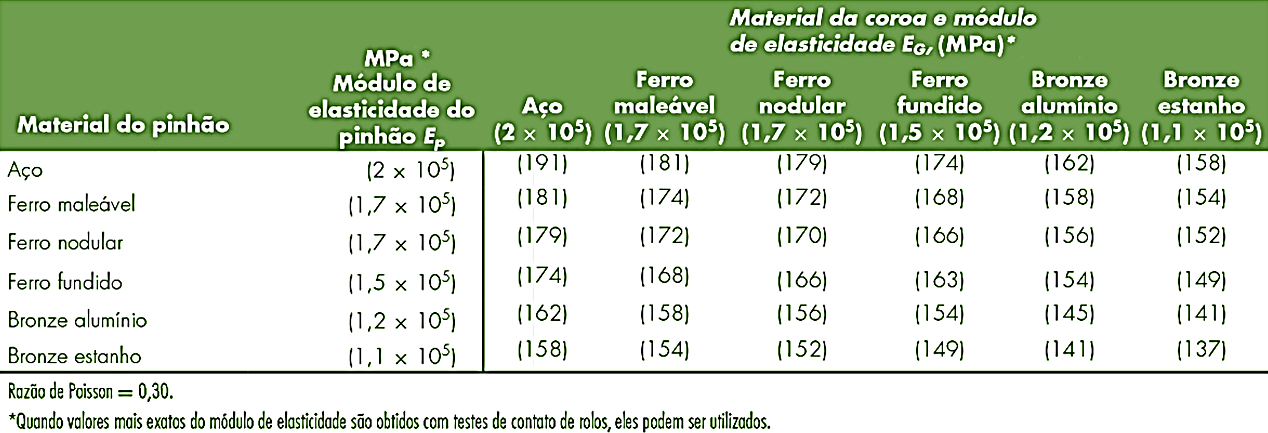
\includegraphics[scale=0.47]{Imagens/Img1.png}\\
    {\footnotesize Fonte: Adaptado de Buday e Nisbett (2014)}
    \label{fig:1}
\end{figure}

\subsubsection*{\texorpdfstring{Carga
tangencial,~\emph{W}\textsuperscript{t}}{Carga tangencial,~Wt}}

{\label{carga-tangencial-wt}}

Na maioria das aplicações de engrenagens, o torque não é constante.
Portanto, a carga tangencial transmitida varia. Para obter valores da
carga tangencial operacional, o projetista deve usar os valores de
potência e velocidade com os quais o dispositivo será acionado. Se a
carga tangencial transmitida for uniforme, então a base de cálculo é
usando a Equação~{\ref{eq:3}}.

\par\null

\begin{equation}
\label{eq:3}
W^t\mathrm{=}\frac{P}{V}\mathrm{=}\frac{T}{r_p}\mathrm{=}\frac{P}{\pi \mathrm{\cdot }D_p\mathrm{\cdot }\omega }
\end{equation}

Onde

\emph{W} \textsuperscript{t} é a carga tangencial, N;

\emph{P} é a potência transmitida, W;

\emph{V} é a velocidade linear, m/s;

\emph{T} é o torque transmitido, N-m;

\emph{r}\textsubscript{p} é o raio primitivo da engrenagem, m;

\emph{D}\textsubscript{p} é o diâmetro primitivo da engrenagem, m;

$\omega$\ é a rotação da engrenagem, rps.

Para encontrar o diâmetro primitivo,~\emph{D}\textsubscript{p}, sabe-se
que tal valor é o produto do módulo e o número de dentes. Por sua vez, a
largura da face, \emph{b}, pode ser obtida da multiplicação do módulo
com constantes de 6 a 16 \hyperref[csl:20]{(Budynas \& Nisbett, 2014}; \hyperref[csl:21]{Mott, 2013)}, e esses módulos são obtidos
da Figura~\ref{fig:2}.

\begin{figure}[!htb]
 \centering
    \caption{Coeficiente de elasticidade padronizado para alguns materiais}
    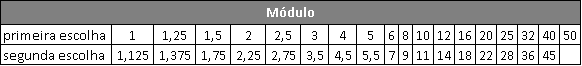
\includegraphics[scale=1]{Imagens/Img2.png}
    {\footnotesize Fonte: Adaptado de Mott (2013)}
    \label{fig:2}
\end{figure}

Quando a carga transmitida não é uniforme, não se deve considerar apenas
o pico de carga e seu número previsto de ciclos, também deve ser
considerada as cargas intermediárias e seu número de ciclos. Nesses
casos, o efeito de fadiga cumulativa do ciclo é considerado na
classificação do conjunto de engrenagens. Um método para calcular o
efeito das cargas sob essas condições é dado na ISO \hyperref[csl:22]{(6336-6, 2006)}.

\subsubsection*{\texorpdfstring{Fator de
sobrecarga,~\emph{K}\textsubscript{o}}{Fator de sobrecarga,~Ko}}

{\label{fator-de-sobrecarga-ko}}

O fator de sobrecarga é destinado a levar em consideração todas as
cargas externas aplicadas à transmissão da engrenagem, além da carga
tangencial,~\emph{W}\textsuperscript{t}, para uma determinada aplicação,
e.g., a existência de choques (impactos) provenientes do torque de
acionamento. O fator de sobrecarga só pode ser estabelecido pelo
engenheiro projetista, após uma considerável experiência de campo.

Para um fator de sobrecarga unitário, pode ser considerada a capacidade
de sustentar um número limitado de até 200\% de ciclos de sobrecarga
momentâneos (geralmente até 4 partidas durante 8 horas, com um pico que
não excede 1 segundo de duração). Sobrecargas momentâneas mais altas ou
mais frequentes devem ser consideradas separadamente.

Ao determinar o fator de sobrecarga, deve-se considerar o fato de que
muitos motores de acionamento e máquinas acionadas, individualmente ou
em combinação, desenvolvem torques de pico momentâneos sensivelmente
maiores do que aquele determinado pela classificação nominal do motor
primário ou da máquina acionada. Existem muitas fontes possíveis de
sobrecarga que devem ser consideradas. Alguns deles são: torques de
partida, velocidades excessivas, variações na operação do sistema e,
alterações nas condições de carga do processo.

Para determinar o fator de sobrecarga, num cenário que não há
experiência a campo do projetista, pode ser usada a Tabela
{\ref{tab:1}}~recomendadas por~\hyperref[csl:21]{(Mott, 2013)}:\selectlanguage{brazil}

\begin{table}[htbp]
    \centering
    \caption{{\label{tab:1} Fator de sobrecarga sugerido}}
    \begin{tabular}{lcccc}
    \hline
&&\textbf{Tipo de máquina acionada} \\\hline
\textbf{Fonte de alimentação} &Uniforme &Choque leve &Choque moderado &Choque pesado\\\hline
Uniforme    &1,00 &1,25 &1,50 &1,75 \\\hline
Choque leve &1,20 &1,40 &1,75 &2,25 \\\hline
Choque moderado & 1,30 & 1,70  & 2,00  & 2,75 \\\hline
    \end{tabular}
\end{table}

Para encontrar o fator de sobrecarga da Tabela {\ref{tab:1}}, devem ser cruzados os valores das colunas: tipo de máquina acionada, com a linha de: fonte de alimentação. Esses valores podem ser obtidos das Figura~\ref{fig:3} e \ref{fig:4}.

\begin{figure}[!htb]
    \centering
    \caption{Condição para máquina acionada}
    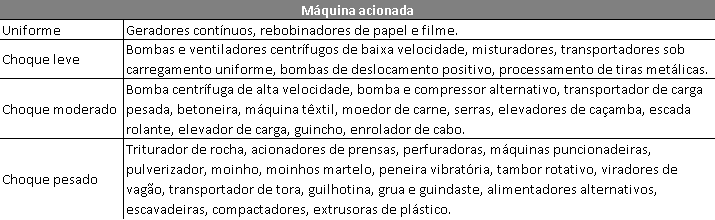
\includegraphics[scale=0.8]{Imagens/Img3.png} \\
    {\footnotesize Fonte: Adaptado de Mott (2013)}
    \label{fig:3}
\end{figure}

\begin{figure}[!htb]
    \centering
    \caption{Condição para fonte de alimentação}
    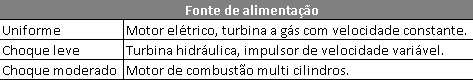
\includegraphics[scale=0.8]{Imagens/Img4.png}\\
    {\footnotesize Fonte: Adaptado de Buday e Nisbett (2014)}
    \label{fig:4}
\end{figure}

\subsubsection*{\texorpdfstring{Fator
dinâmico,~\emph{K}\textsubscript{V}}{Fator dinâmico,~KV}}

{\label{fator-dinuxe2mico-kv}}

O fator dinâmico,~\emph{K}\textsubscript{v}, é responsável pelas cargas
dos dentes da engrenagem geradas internamente, que são induzidas pela
ação do engrenamento não conjugadas totalmente (não harmonizadas). Mesmo
que o torque e a velocidade de entrada sejam constantes, pode haver uma
vibração significativa das massas das engrenagens e, portanto, haverá
forças dinâmicas nos dentes. Essas forças resultam das acelerações
relativas entre as engrenagens, pois elas vibram em resposta a uma
excitação conhecida como ''erro de transmissão''. Idealmente, um
conjunto de engrenagens teria uma taxa de velocidade uniforme entre a
rotação de entrada e saída. O ``erro de transmissão'' é definido como o
desvio do movimento angular relativo uniforme do par de engrenagens. É
influenciado por todos os desvios existentes da forma geométrica do
dente da engrenagem em relação ao espaçamento ideal. O ``erro de
transmissão'' pode ser influenciado por:

\begin{itemize}
\tightlist
\item
  Variações na fabricação da engrenagem, no espaçamento entre dentes
  (passo), perfil da involuta (tolerância geométrica), e afastamentos
  (tolerância dimensional).
\item
  Variação de rigidez nos dentes da engrenagem à medida que os dentes
  passam pelo engrenamento.
\item
  Deflexões elásticas que fogem de uma carga projetada.
\item
  Desbalanceamento dinâmico das engrenagens e/ou eixos.
\item
  Desgaste excessivo, não projetadas, e deformação plástica do perfil do
  dente da engrenagem.
\item
  Desalinhamento do eixo influenciado pelas cargas e deformações
  térmicas das engrenagens, dos eixos, mancais, variações de fabricação,
  ou simplesmente erro de montagem.
\item
  Excitação induzida por fricção entre dentes.
\end{itemize}

A Figura {\ref{fig:5}} mostra os fatores dinâmicos que
podem ser utilizados na ausência de conhecimento específico das cargas
dinâmicas.~Devido à natureza aproximada das curvas empíricas e à falta
de valores de tolerância medidos no estágio de projeto, as curvas de
fator dinâmico devem ser selecionadas com base na experiência dos
processos de fabricação e das considerações operacionais de projeto.

Segundo \hyperref[csl:21]{(Mott, 2013)}, por meio de uma medição tangencial no
diâmetro primitivo dos dentes da engrenagem, podem ser obtidas algumas
precisões do seu perfil. Assim, quando aceita a 3 medições com um
Engrenômetro, pode considerar-se que o Número de nível de precisão
(\emph{A}\textsubscript{v}) é de 12 a 10 e pode ser considerado de baixa
precisão. Se a medição é aceita em 5 medições, considera-se
um~\emph{A}\textsubscript{v} de 9 a 6 e pode ser considerado de média
precisão. Para 9 medições com sucesso, considera-se
um~\emph{A}\textsubscript{v} de 5 a 2 e pode ser considerado de alta
precisão. Para~~\emph{A}\textsubscript{v}~abaixo de 2, é considerado
muito preciso.

Para maiores detalhes da escolha de \emph{A}\textsubscript{v} = 6
a~\emph{A}\textsubscript{v} = 12 consultar a norma
ANSI/AGMA~\hyperref[csl:23]{(2015-A01, 2002)}.\selectlanguage{brazil}

\begin{figure}[!htb]
    \centering
    \caption{Curvas do número de nível de precisão}
    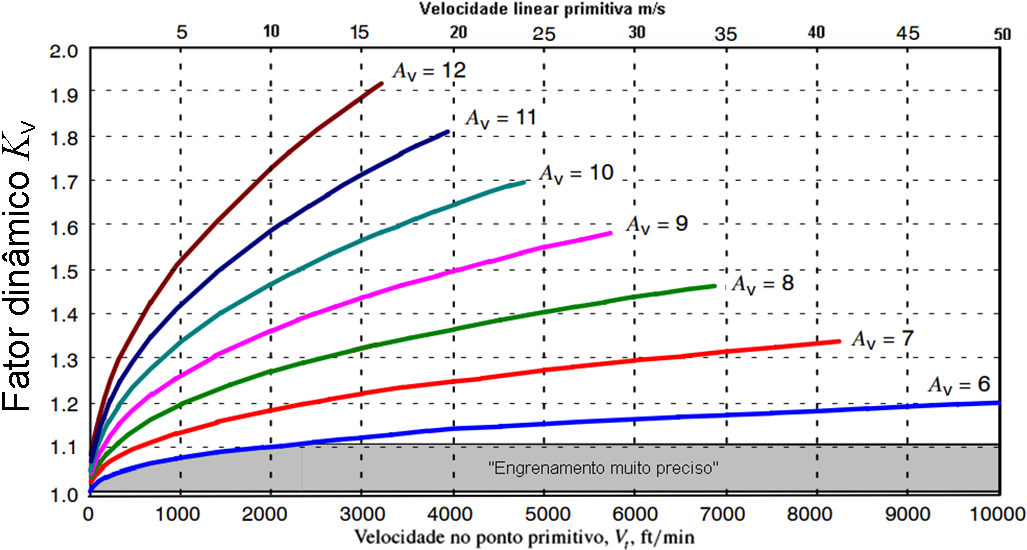
\includegraphics[scale=0.57]{Imagens/Img5.png}\\
    {\footnotesize Fonte: Adaptado de ANSI/AGMA 2101-D04 (2016)}
    \label{fig:5}
\end{figure}

As curvas da Figura {\ref{fig:5}} cruzadas com a
velocidade no ponto primitivo da engrenagem servem para encontrar o
fator dinâmico. Segundo \hyperref[csl:21]{(Mott, 2013)}, sabendo o número de nível de
precisão (\emph{A}\textsubscript{v}), podem ser usadas as equações
{\ref{eq4}}, {\ref{eq5}} e~{\ref{eq6}} para encontrar também o fator dinâmico.

\begin{equation}
    \label{eq4}
    K_{\mathrm{V}}\mathrm{=}{\left[\frac{C}{C+\sqrt{V}}\right]}^{-B}
\end{equation}

\begin{equation}
    \label{eq5}
    B=0,25{(A_{\mathrm{v}}-5,0)}^{{2}/{3}}
\end{equation}

\begin{equation}
    \label{eq6}
    C=3,5637+3,9914(1,0-B)
\end{equation}

Quando a engrenagem é fabricada usando controles de processo que
fornecem precisões nos dentes, ou seja, engrenagens muito precisas, ou
quando as técnicas de fabricação e de projeto garantem um baixo ``erro
de transmissão'', podem ser considerados valores
de~\emph{K}\textsubscript{v}~de 1.02 a 1.11, essa escolha depende da
experiência do projetista. Para usar esses valores, a engrenagem deve
ser mantida em alinhamento preciso e lubrificada adequadamente, para que
sua precisão seja mantida na vida útil de operação.

\hyperref[csl:21]{(Mott, 2013)}, apresenta alguns equipamentos na Figura~\ref{fig:6}, que auxilia na rápida seleção do número
de nível de precisão (\emph{A}\textsubscript{v}), segundo a aplicação de
operação do conjunto de engrenagens.\selectlanguage{brazil}

\begin{figure}[!htb]
    \centering
    \caption{Aplicação para encontrar o número de nível de precisão}
    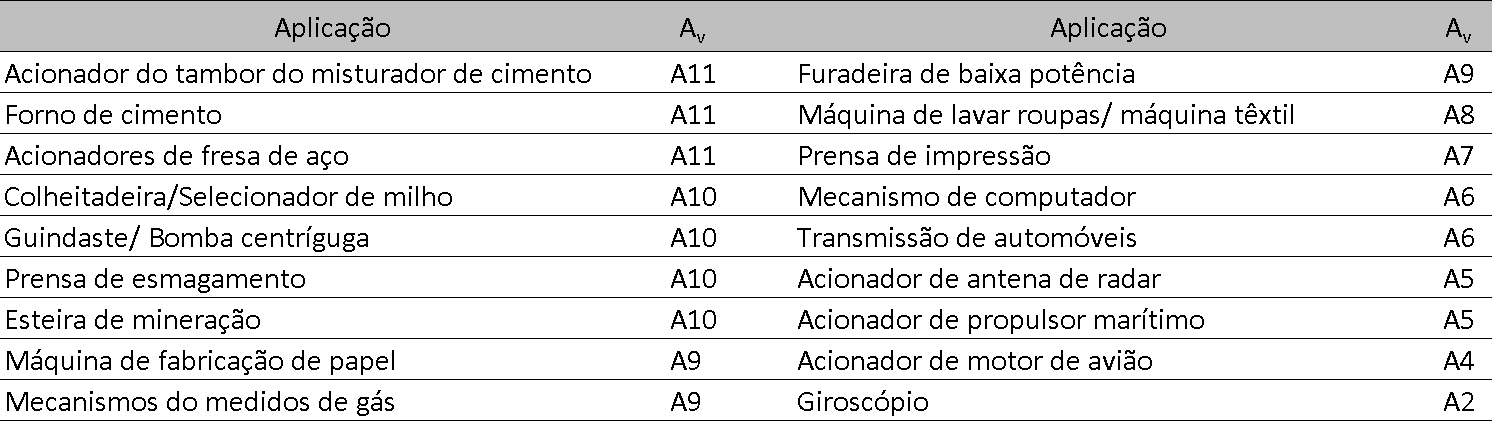
\includegraphics[scale=0.4]{Imagens/Img6.png}\\
    {\footnotesize Fonte: Adaptado de Mott (2013)}
    \label{fig:6}
\end{figure}

As curvas podem ser extrapoladas além dos pontos finais mostrados na
Figura \ref{fig:5}, com base na experiência e na
consideração cuidadosa dos fatores que influenciam a carga dinâmica.

Se uma frequência específica da excitação do ``erro de transmissão''
estiver próxima da frequência natural do sistema de massa-mola da
engrenagem, ou algum múltiplo da frequência natural, como 2 ou 3, uma
vibração ressonante poderá causar forças dinâmicas elevadas nos dentes
devido a grandes deslocamentos relativos das massas da engrenagem. O
fator dinâmico, \emph{K}\textsubscript{v}, não leva em consideração a
ressonância do par de engrenagens, e a operação nesse regime deve ser
evitada.

Além disso, devido à alta resistência à flexão dos eixos das
engrenagens, as frequências naturais de vibração lateral dos eixos
geralmente são muito mais altas que as velocidades de operação. Para
engrenagens de alta velocidade, no entanto, recomenda-se que as
velocidades críticas do eixo sejam analisadas para garantir que elas
sejam bem removidas da faixa de velocidade operacional. O fator
dinâmico, \emph{K}\textsubscript{v}, não considera as cargas dinâmicas
dos dentes devido a este modo de vibração.

\subsubsection*{\texorpdfstring{Fator de
tamanho,~\emph{K}\textsubscript{s}}{Fator de tamanho,~Ks}}

{\label{fator-de-tamanho-ks}}

O fator de tamanho refere-se à não uniformidade das propriedades do
material e depende principalmente de:Tamanho do dente

\begin{itemize}
\tightlist
\item
  Diâmetro das partes
\item
  Proporção entre tamanho do dente e diâmetro da peça
\item
  Largura da face
\item
  Proporção da profundidade em relação ao tamanho do dente
\item
  Dureza e tratamento térmico do material
\end{itemize}

O fator de tamanho pode ser considerado 1,0 para a maioria das
engrenagens, desde que seja feita uma escolha adequada de aço para o
tamanho da peça e, seu tratamento térmico e processo de endurecimento.

\hyperref[csl:20]{(Budynas \& Nisbett, 2014)}~propõem que para encontrar o fator de tamanho
K\textsubscript{S} pode ser adotado o recíproco do fator de
tamanho~\emph{k}\textsubscript{b} usado na equação de Lewis. Assim,
dependendo da largura da face podem ser usada a
equação~{\ref{eq7}} ou~{\ref{eq8}}:

Se a largura da face for de 2,79 a 51 mm, Equação
{\ref{eq7}}.

\begin{equation}
    \label{eq7}
K_{\mathrm{S}}\mathrm{=}\frac{\mathrm{1}}{\mathrm{1,1833}{\left(b\mathrm{\cdot }m\mathrm{\cdot }\sqrt{Y}\right)}^{\mathrm{-}\mathrm{0,0535}}}
\end{equation}

Se a largura da face for de 52 a 254 mm, Equação~{\ref{eq8}}.

\begin{equation}
    \label{eq8}
K_{\mathrm{S}}\mathrm{=}\frac{\mathrm{1}}{\mathrm{1,4098}{\left(b\mathrm{\cdot }m\mathrm{\cdot }\sqrt{Y}\right)}^{\mathrm{-}\mathrm{0,0785}}}
\end{equation}

Para encontrar a constante Y que é o fator de forma de Lewis, para
engrenagens de aço e ângulo de pressão (ou contato) 20°, devem ser
usados os valores contidos na Figura \ref{fig:7}.\selectlanguage{brazil}

\begin{figure}[!htb]
    \centering
    \caption{Valores do fator de forma Y de Lewis para angulo de pressão 20°}
    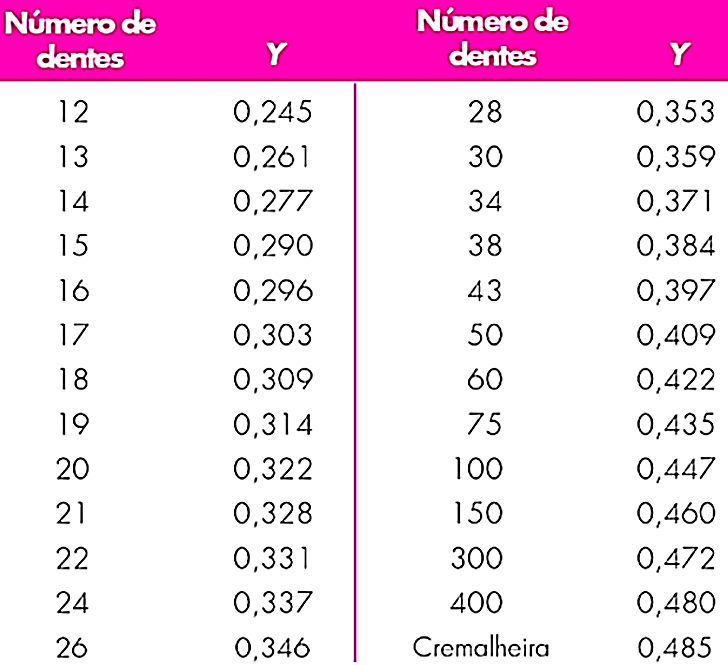
\includegraphics[scale=0.9]{Imagens/Img7.png}\\
    {\footnotesize Fonte: Adaptado de Buday e Nisbett (2014)}
    \label{fig:7}
\end{figure}

Segundo \hyperref[csl:21]{(Mott, 2013)}, também pode ser considerado o fator de
tamanho em função do módulo usado, conforme apresentado na Figura
{\ref{fig:8}}.

\begin{figure}[!htb]
    \centering
    \caption{Fator de tamanho segundo o módulo}
    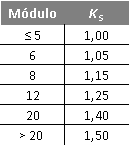
\includegraphics[scale=0.9]{Imagens/Img8.png}\\
    {\footnotesize Fonte: Adaptado de Mott (2013)}
    \label{fig:8}
\end{figure}

\subsubsection*{\texorpdfstring{Fator de distribuição de
carga,~\emph{K}\textsubscript{H}}{Fator de distribuição de carga,~KH}}

{\label{fator-de-distribuiuxe7uxe3o-de-carga-kh}}

O fator de distribuição de carga, modifica a classificação das equações
de tensão AGMA para refletir a distribuição não uniforme da carga ao
longo da linha de contato (flanco no diâmetro primitivo). A quantidade
de não uniformidade da distribuição de carga causada depende das
seguintes influências:

\begin{itemize}
\tightlist
\item
  Variação no processo de fabricação das engrenagens;
\item
  Alinhamento, geometria de perfil, espaçamento e desvios nas
  engrenagens pinhão e coroa;
\item
  Coroamento no dente e/ou alívio no flanco do adendo;
\item
  Variações de montagem das engrenagens;
\item
  Alinhamento dos eixos, na rotação do diâmetro primitivo da engrenagem,
  influenciados pela folga de precisão de concentricidade dos mancais;
\item
  Deflexões devido a cargas aplicadas;
\item
  Deflexões elásticas no dente da engrenagem;
\item
  Deflexões elásticas do corpo da engrenagem;
\item
  Deflexões elásticas do eixo, mancais de rolamento ou de deslizamento e
  estrutura que suportam as engrenagens;
\item
  Distorções devido a efeitos centrífugos;
\item
  Expansão térmica e distorção das engrenagens devido a gradientes de
  temperatura;
\item
  Gradientes de temperatura no mancal causando eixos não paralelos;
\item
  Distorção centrífuga das engrenagens devido a altas velocidades.
\end{itemize}

O fator de distribuição de carga da face do dente é responsável pela
distribuição não uniforme da força ao longo do flanco. A magnitude do
fator de distribuição da carga da face é definida como a intensidade do
pico de carga dividida pela intensidade média da carga em toda a largura
da face.

Quando a engrenagem está em balanço, deve-se considerar a deflexão do
eixo e as folgas dos mancais. No entanto, em sistemas que a engrenagem
não está em balanço, o eixo e mancais devem estar rígidos o suficiente
para suportar os momentos de flexão causados pelas forças do
engrenamento. Além disso, deve se seguir as folgas recomendadas pelos
fabricantes de mancais, já que as folgas excessivas afetam o contato da
engrenagem tão igual como uma montagem errada das engrenagens. Por outro
lado, a engrenagem com um deslocamento mais próximo a um dos mancais
pode também agravar a deflexão não desejada, e esse efeito é tratado
pelo fator de carga de deflexão (\(K_{\text{Hpm}}\)).

Para projetos de engrenagens relativamente rígidos com engrenagens
montadas entre rolamentos (engrenagem não suspensa) e relativamente
livres de fatores externos que causem deflexões não projetadas, a
Equação {\ref{eq9}} pode ser usado:

\par\null

\begin{equation}
    \label{eq9}
K_{\mathrm{H}}\mathrm{=1.0+}K_{\mathrm{Hmc}}\left(K_{\mathrm{Hpf}}{\mathrm{\cdot }K}_{\mathrm{Hpm}}\mathrm{+}K_{\mathrm{Hma}}\mathrm{\cdot }K_{\mathrm{He}}\right)
\end{equation}

Onde

\(K_{\text{Hmc}}\)~é o fator de formato da face do dente;

\(K_{\text{Hpf}}\)~é o fator de proporção do pinhão;

\(K_{\text{Hpm}}\)~é o fator de carga de deflexão;

\(K_{\text{Hma}}\)~é o fator de alinhamento de engrenamento;

\(K_{\text{He}}\)~é o fator de ajuste.

O fator de formato da face do dente,~\(K_{\text{Hmc}}\), modifica a
intensidade de carga máxima quando é aplicado coroamento ou alívio na
ponta do adendo. A norma AGMA, considera apenas o impacto do coroamento,
para o cálculo de alívio na ponta do adendo podem ser consultados
pesquisas específicas sobre esse assunto~\hyperref[csl:12]{(Maper et al., 2019}; \hyperref[csl:9]{Wen et al., 2019}; \hyperref[csl:11]{Zhan et al., 2015)}.

Para entender o formato de uma engrenagem com coroamento no dente e
assumir o valores para \(K_{\text{Hmc}}\), deve ser considerada a Figura
{\ref{fig:9}}.\selectlanguage{brazil}

\begin{figure}[!htb]
    \centering
    \caption{Coroamento e valores para fator de forma da face do dente}
    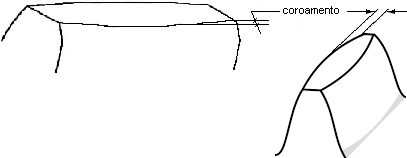
\includegraphics[scale=0.8]{Imagens/Img9.png}\\
   {\footnotesize Fonte: Adaptado de ANSI/AGMA 2101-D04 (2016)}
    \label{fig:9}
\end{figure}

\begin{equation}
K_{\text{Hmc}}\left\{\begin{matrix}1.0\ \ \ \ \ \ \ \ \ \ \ \ \ \ \ \ \ \  \ \ \ \ \ \ \ \ \ \ \ \ \ \  \text{para\ dente\ sem\ coroamento}\\
0.8\ \selectlanguage{Brazil}\text{para\ dente\ coroado\ ou\ com\ correção de desvio}\\
\end{matrix}\right.\ \nonumber \\
\end{equation}

O dente coroado pode ajudar a concentrar a carga em direção do centro do
dente, mitigando ruído e vibração. Mas a coroação excessiva pode
aumentar a tensão por contato numa região pontual e ocasionar falhas que
afetam a vida útil remanescente do sistema \hyperref[csl:24]{(Nu{\~{n}}ez \& Borsato, 2017}; \hyperref[csl:25]{Nu{\~{n}}ez \& Borsato, 2018)}.

O fator de proporção do pinhão, \(K_{\text{Hpf}}\), responde à deflexões
no dente devido à carga. Essa deflexão é normalmente mais elevada para
grandes larguras na face do dente. O \(K_{\text{Hpf}}\) pode ser
encontrado com a relação da largura da face (\emph{b)} e o diâmetro
primitivo (\emph{D}\textsubscript{p}), apresentada a
seguir.

\begin{equation}
K_{\text{Hpf}}\left\{\begin{matrix} \text{Se}\ b\leq 25\ \text{mm},\ \ \ \ \ \ \ \ \ \ \ \ \ \ \ \ \ \ \ \ \ \ \ \ \ \ \ \ \ \ \ \ \ \ \ \ \ \ \ \ \ \ \ \ \ \ \ \ \ \ \ \ \ \ \ \ \ \ \ \ \ \ \ \ \ \ \ \ \ \ \ \ \ \ \ \ \ \ \text{então}\ \frac{b}{10\cdot D_{P}}-0,025\\\\\text{Se}\ 25\ <b\leq 432\ \text{mm},\ \ \ \ \ \ \ \ \ \ \ \ \ \ \ \ \ \ \ \ \ \ \ \ \ \ \ \ \ \ \ \ \ \ \ \ \ \ \ \text{então}\ \frac{b}{10\cdot D_{P}}-0,0375+0,000492\cdot b\\\\\text{Se}\ 432\ <b\leq 1\ 020,\ \ \ \ \ \ \ \ \text{então}\ \frac{b}{10\cdot D_{P}}-0,1109+0,000815\cdot b-0,000000353\cdot b^{2}\\
\end{matrix}\right.\ \nonumber \\
\end{equation}

Para valores de \(\frac{b}{10\cdot D_{P}}\) inferiores a 0,05, assuma o \(K_{\text{Hpf}}\) igual a 0,05.

Também, pode ser encontrado o \(K_{\text{Hpf}}\) considerando as curvas
da Figura {\ref{fig:10}}, para tal deve ser cruzado o
valor de \emph{b} com a relação~\emph{b}/\emph{D}\textsubscript{p}:\selectlanguage{brazil}

\begin{figure}[!htb]
    \centering
    \caption{Curvas para encontrar o fator de proporção do pinhão}
    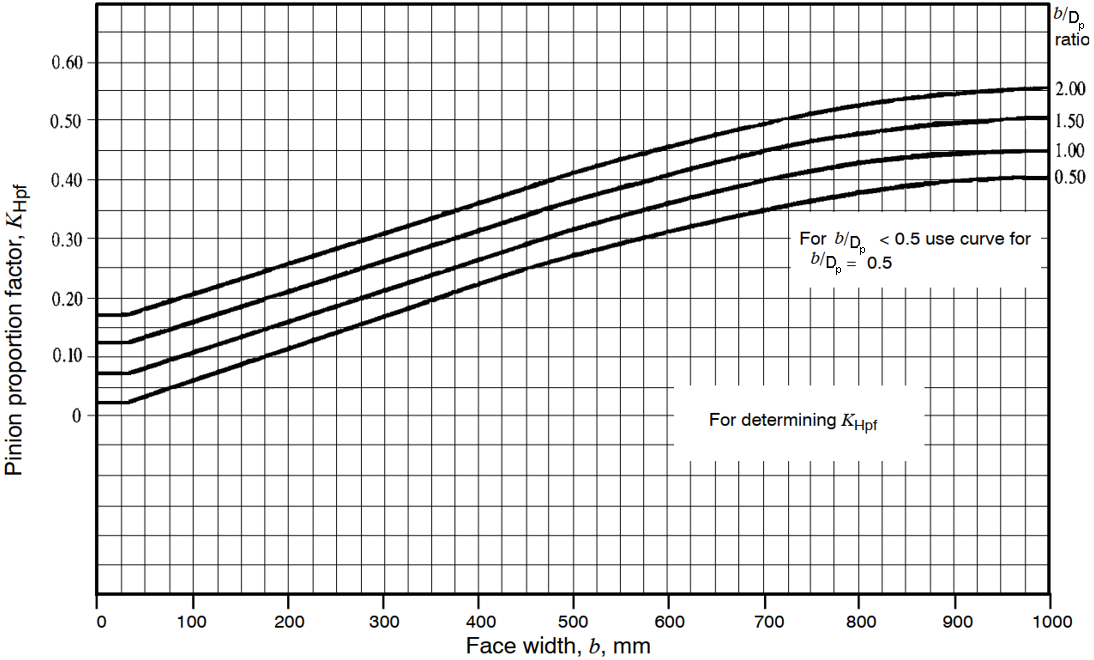
\includegraphics[scale=0.55]{Imagens/Img10.png}\\
    {\footnotesize Fonte: Adaptado de ANSI/AGMA 2101-D04 (2016)}
    \label{fig:10}
\end{figure}

O fator de carga de flexão \emph{K}\textsubscript{Hpm} altera
o~\emph{K}\textsubscript{Hpf}, com base na localização do pinhão ao
longo do eixo de transmissão, especificamente a posição da engrenagem
entre os dois mancais de apoio, conforme representado na Figura
{\ref{fig:11}}.\selectlanguage{brazil}

\begin{figure}[!htb]
    \centering
    \caption{Posição da engrenagem no eixo de transmissão}
    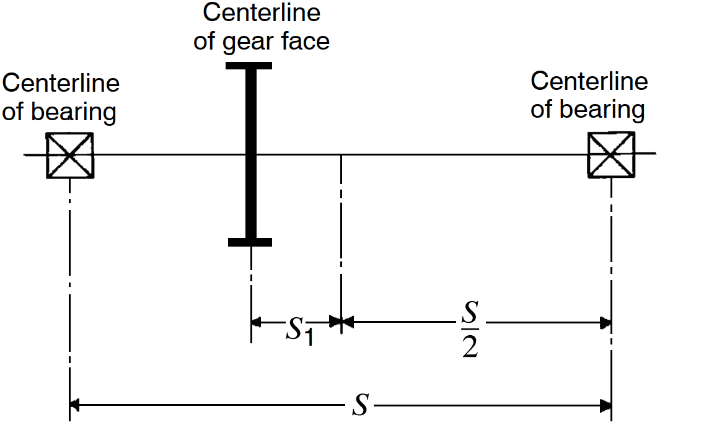
\includegraphics[scale=0.9]{Imagens/Img11.png}\\
    {\footnotesize Fonte: Adaptado de ANSI/AGMA 2101-D04 (2016)}
    \label{fig:11}
\end{figure}

Dependendo se a posição da engrenagem em relação aos dois mancais de
apoio for maior ou menor de 17,5\%, pode ser assumido o valor
para~\emph{K}\textsubscript{Hpm}, conforme:

\begin{equation}
K_{\text{Hpm}}\left\{\begin{matrix}1.0\ para\ pinhao\ montado\ com\ \left(\frac{S_{1}}{S}\right)<0.175\\\\
1.1\ para\ pinhao\ montado\ com\ \left(\frac{S_{1}}{S}\right)\geq 0.175\\
\end{matrix}\right.\ \nonumber \\
 \end{equation}

Onde

\emph{S}\textsubscript{1}: é o deslocamento do pinhão; isto é, a
distância em relação ao centro do vão dos mancais;

\emph{S} : é o vão entre mancais; ou seja, a extensão entre as linhas de
centro dos mancais.

O fator de alinhamento de engrenamento, \emph{K}\textsubscript{Hma},
avalia a influência do desalinhamento de um eixo de transmissão e o
efeito que este gera na rotação das engrenagens, especificamente no
diâmetro primitivo. Segundo a norma AGMA, para encontrar esse valor pode
ser encontrado cruzando a largura da face,~\emph{b,} com uma das 4
curvas que estão relacionadas à rigidez dos mancais, apresentadas na
Figura {\ref{fig:12}}.\selectlanguage{brazil}

\begin{figure}[!htb]
    \centering
    \caption{Curvas para o fator de alinhamento de engrenamento}
    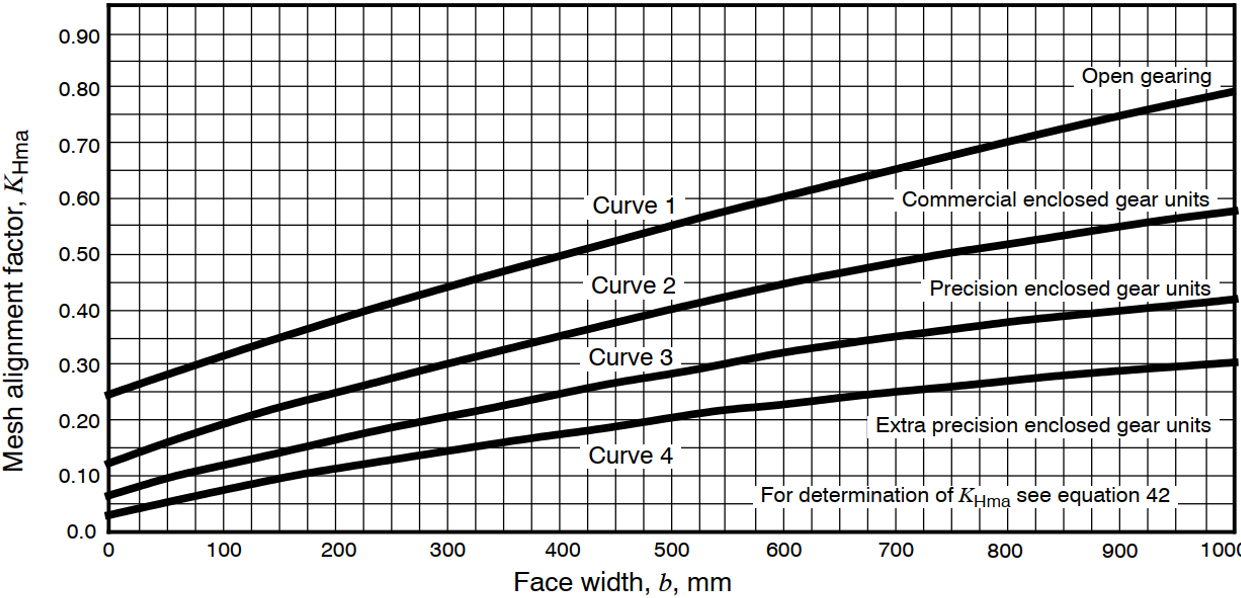
\includegraphics[scale=0.47]{Imagens/Img12.png}\\
    {\footnotesize Fonte: Adaptado de ANSI/AGMA 2101-D04 (2016)}
    \label{fig:12}
\end{figure}

A norma AGMA não consideram que a causa desse desalinhamento seja por
deformação elástica. E, outra forma de encontrar o fator de alinhamento
é usando a Equação {\ref{eq10}}. Para atribuir um valor
às constantes~\emph{A, B} e~\emph{C} da Equação
{\ref{eq10}} e encontrar o~\emph{K}\textsubscript{Hma},
deve-se identificar as características que cada curva representa com
base na precisão dos efeitos nas engrenagens e seu consequente
desalinhamento.

\begin{equation}
    \label{eq10}
K_{\mathrm{Hma}}\mathrm{=}A\mathrm{+}B\left(b\right)\mathrm{+}C{\mathrm{(}b\mathrm{)}}^{\mathrm{2}}
\end{equation}

~Segundo \hyperref[csl:21]{(Mott, 2013)}, cada curva considera o tipo de montagem dos
mancais:

\begin{itemize}
\tightlist
\item
  \textbf{Curva 1 - Engrenagem aberta:} quando os mancais são montados
  na estrutura da própria máquina;
\item
  \textbf{Curva 2 - Engrenagem fechada industrial/comercial:} os mancais
  são montados numa estrutura especial, proporcionando uma melhor
  rigidez;
\item
  \textbf{Curva 3 - Engrenagem fechada de precisão:} mancais montados
  numa estrutura especial e com tolerâncias dimensionais;
\item
  \textbf{Curva 4 - Engrenagem fechada de alta precisão:} os mancais
  montados possuem uma tolerância dimensional minuciosa, normalmente há
  ajustes na montagem para conseguir um alinhamento muito preciso no
  engrenamento.
\end{itemize}

Os valores a serem considerados nas constantes \emph{A, B} e
\emph{C~}são apresentada na Figura {\ref{fig:13}}.\selectlanguage{brazil}

\begin{figure}[!htb]
    \centering
    \caption{Valores das constantes do fator de alinhamento}
    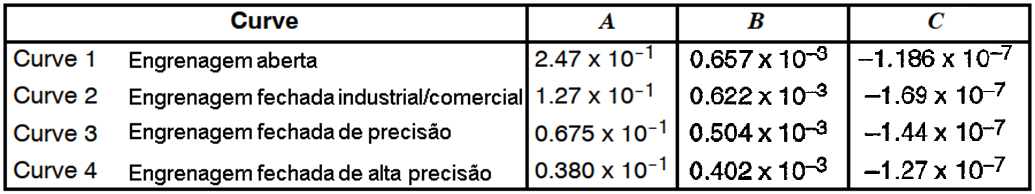
\includegraphics[scale=0.5]{Imagens/Img13.png}\\
    {\footnotesize Fonte: Adaptado de ANSI/AGMA 2101-D04 (2016)}
    \label{fig:13}
\end{figure}

O fator de ajuste, \emph{K}\textsubscript{He}, é usado para modificar o
fator de alinhamento de engrenamento. Os seguintes valores são sugeridos
para o fator de correção do alinhamento de engrenamento:

\begin{equation}
K_{\text{He}}\left\{\begin{matrix}
0.8\ \ \ \ \ \  \ \ \ \ \ \ \ \ \ \ \ \ \ \ \ \ \ \ \ \ \ \ \ \ quando\ a\ engrenagem\ e\ ajustada\ na\ montagem\\
0.8\ quando\ a\ compatibilidade\ da\ engrenagem\ e\ melhorada\ lapidando\\
1.0\ \ \ \ \ \ \ \ \ \ \ \ \ \ \ \ \ \ \ \ \ \ \ \ \ \ \ \ \ \ \ \ \ \ \ \ \ \ \ \ \ \ \ \ \ \ \ \ \ \ \ \ \ \ \ \ \ \ \ \ \ \ \ \ \ \ \ \ para\ todos\ os\ outros\ casos\\
\end{matrix}\right.\ \nonumber \\
\end{equation}

\subsubsection*{\texorpdfstring{Fator de condição
superficial,~\emph{Z}\textsubscript{R}}{Fator de condição superficial,~ZR}}

{\label{fator-de-condiuxe7uxe3o-superficial-zr}}

O fator de condição superficial, \emph{Z}\textsubscript{R}, é usado
apenas na fórmula de resistência ao crateramento e depende de:

\begin{itemize}
\tightlist
\item
  Acabamento da superfície de rebarbação, lapidação, retífica, e
  jateamento por granalha;
\item
  Tensão residual;
\item
  Efeitos de plasticidade (endurecimento).
\end{itemize}

Os fatores de condição superficial para dentes de engrenagem ainda não
foram estabelecidos para casos em que há um efeito de acabamento
superficial prejudicial. Nesses casos, algum
\emph{Z}\textsubscript{R~}maior a 1,0 pode ser usado dependendo da
experiência do engenheiro projetista. O \emph{Z}\textsubscript{R} pode
ser tomado como 1,0 desde que a condição de superfície apropriada seja
alcançada.

\subsubsection*{\texorpdfstring{Fator geométrico ao
crateramento,~\emph{Z}\textsubscript{I}}{Fator geométrico ao crateramento,~ZI}}

{\label{749784}}

O fator de geometria,~\emph{Z}\textsubscript{I}, avalia os raios de
curvatura do perfil do dente em contato, com base na forma da sua
involuta. Esses raios são usados para avaliar a tensão de contato de
Hertz no flanco do dente. Os efeitos das proporções modificadas dos
dentes e do compartilhamento de carga são considerados.

Segundo \hyperref[csl:21]{(Mott, 2013)} o fator geométrico para resistência ao
crateramento pode ser obtido da Equação~{\ref{eq11}}.

\begin{equation}
\label{eq11}
Z_I\mathrm{=}C_c\mathrm{\cdot }C_x
\end{equation}

Onde

\emph{C\textsubscript{c}} é o fator de curvatura na linha primitiva;

\emph{C\textsubscript{x}} é o fator para ajuste da altura específica do
LPSTC (ponto extremo inferior de contato de um dente, abaixo da linha
primitiva).

Assim, \emph{Z}\textsubscript{I}~pode ser obtido usando as
equações~{\ref{eq12}},~{\ref{eq13}},~{\ref{eqx}},~{\ref{eq14}},~{\ref{eq16}}~e~{\ref{eq17}}.

\begin{equation}
\label{eq12}
C_c\mathrm{=}\frac{{\mathrm{cos} \theta \ }\mathrm{\cdot }{\mathrm{sen} \theta \ }}{\mathrm{2}}\mathrm{\cdot }\frac{i}{i\mathrm{+1}}
\end{equation}
\\
\begin{equation}
\label{eq13}
C_x\mathrm{=}\frac{\mathrm{(}C_{\mathrm{1}}\mathrm{-}C_{\mathrm{3}}\mathrm{+}C_{\mathrm{4}}\mathrm{)(}C_{\mathrm{2}}\mathrm{+}C_{\mathrm{3}}\mathrm{-}C_{\mathrm{4}}\mathrm{)}}{C_{\mathrm{1}}\mathrm{\cdot }C_{\mathrm{2}}}
\end{equation}
\\
\begin{equation}
\label{eqx}
C_1=\frac{\mathrm{(}N_P\mathrm{\cdot }{\mathrm{sen} \theta \mathrm{)}\ }}{\mathrm{2}}
\end{equation}
\\
\begin{equation}
\label{eq14}
C_{\mathrm{2}}\mathrm{=}C_1{\cdot }i
\end{equation}
\\
\begin{equation}
\label{eq16}
C_{\mathrm{3}}\mathrm{=}\pi \mathrm{\cdot }{\mathrm{cos} \theta \ }
\end{equation}
\\
\begin{equation}
\label{eq17}
C_{\mathrm{4}}\mathrm{=0,5}\left[\sqrt{{\left(N_P\mathrm{+2}\right)}^{\mathrm{2}}\mathrm{-}{\left(N_P\mathrm{\cdot }{\mathrm{cos} \theta \ }\right)}^{\mathrm{2}}}\mathrm{-}\sqrt{N^{\mathrm{2}}_P\mathrm{-}{\left(N_P\mathrm{\cdot }{\mathrm{cos} \theta \ }\right)}^{\mathrm{2}}}\right]
\end{equation}

Onde o N\textsubscript{P} é o número de dentes do pinhão. Também pode
ser encontrado o fator geométrico de resistência ao crateramento no
gráfico da Figura~{\ref{fig:14}},~\hyperref[csl:21]{(Mott, 2013)}.
Para este fator deve ser considerada à relação de transmissão
(\emph{i}).\selectlanguage{brazil}

\begin{figure}[!htb]
    \centering
    \caption{Fator geométrico de resistência ao crateramento para ângulo de pressão 20°}
    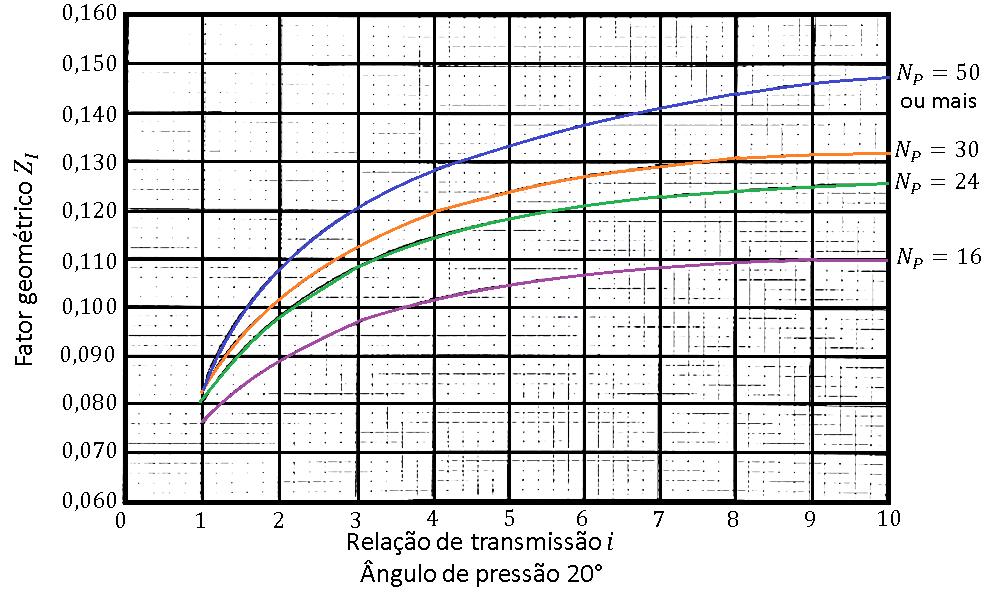
\includegraphics[scale=0.6]{Imagens/Img14.png}\\
    {\footnotesize Fonte: Adaptado de Mott (2013)}
    \label{fig:14}
\end{figure}

\subsection*{\texorpdfstring{Fator de segurança AGMA ao
contato,~\emph{S}\textsubscript{H}}{Fator de segurança AGMA ao contato,~SH}}

{\label{fator-de-seguranuxe7a-agma-ao-contato-sh}}

Para o fator de segurança AGMA ao contato, recomenda-se que esse valor
esteja no intervalo de 1 a 1,5~\hyperref[csl:21]{(Mott, 2013)}. A
Equação~{\ref{eq18}} serve para encontrar esse fator de
segurança que garante uma resistência ao crateramento de projeto,
lembrando que a tensão ao contato, $\sigma_H$, já foi abordada.

\begin{equation}
\label{eq18}
S_{\mathrm{H}}\mathrm{=}\frac{Z_{\mathrm{N}}\mathrm{\cdot }Z_{\mathrm{W}}}{Y_{\theta }\mathrm{\cdot }Y_{\mathrm{Z}}}\cdot \frac{{\sigma }_{\mathrm{HP}}}{{\sigma }_{\mathrm{H}}}
\end{equation}

Onde

\(S_{H}\) é o fator de segurança AGMA ao contato;

\(\sigma_{\text{HP}}\) é o número ao contato permitido
AGMA,\(\frac{N}{\text{mm}^{2}}\);

\(\sigma_{H}\) é a tensão ao contato AGMA, \(\frac{N}{\text{mm}^{2}};\)

\(Z_{N}\) é o fator do ciclagem de tensão para resistência ao
crateramento;

\(Z_{W}\) é o fator de razão de dureza para resistência ao
crateramento;

\(Y_{\theta}\) é o fator de temperatura;

\(Y_{Z}\) é o fator de confiabilidade.

O \(\sigma_{\text{HP}}\) não tem relação com a resistência ao escoamento
(\emph{S}\textsubscript{y})\emph{,} resistência última
(\emph{S}\textsubscript{ut}) ou resistência ao limite de fadiga
(\emph{S}\textsubscript{e}). Deve ser usado apenas para fator de
segurança AGMA.

\subsubsection*{\texorpdfstring{Fator de ciclagem de tensão para
resistência ao crateramento,
Z\textsubscript{N}}{Fator de ciclagem de tensão para resistência ao crateramento, ZN}}

{\label{fator-de-ciclagem-de-tensuxe3o-para-resistuxeancia-ao-crateramento-zn}}

O fator de ciclagem por contato, \emph{Z}\textsubscript{N}, ajusta o
número de tensão ao contato permitido para o número necessário de ciclos
de operação. Para os fins desta norma, \emph{n}\textsubscript{L}, é o
número de ciclos de tensão e é definido como o número de contatos de
engrenamento, sob carga, no dente da engrenagem sendo analisada. Os
números de tensão permitido pela AGMA são estabelecidos para ciclos de
carga acima de 10\textsuperscript{7} de forma unidirecional no dente da
engrenagem. Para tal, pode ser usada a Equação
{\ref{eq19}}, obtida com 99\% de confiabilidade, que é
a parte superior da região sombreada na Figura
{\ref{fig:16}}.

\begin{equation}
\label{eq19}
Z_{\mathrm{N}}\mathrm{=1,4488}\mathrm{\cdot }{n_{\mathrm{L}}}^{\mathrm{-}\mathrm{0,023}}
\end{equation}

Para encontrar o número de ciclos de tensão deve ser usada a Equação
{\ref{eq20}}.

\begin{equation}
\label{eq20}
n_L\mathrm{=60}\mathrm{\cdot }L\mathrm{\cdot }\omega \mathrm{\cdot }q
\end{equation}

Onde

\(n_{L}\) é o número de ciclos de tensão;

\(L\) é a vida nominal projetada, (em horas);

\(\omega\) é a rotação, rpm;

\(q\) é o número de contatos por revolução.

A vida nominal a ser considerada no projeto da engrenagem depende da
experiência do engenheiro projetista. Para auxiliar na definição de vida
nominal, \hyperref[csl:21]{(Mott, 2013)}, apresenta uma lista com algumas horas a
serem consideradas para o projeto. Essa recomendação de horas de
trabalho é uma convenção entre informações provenientes de especialistas
da indústria e cientistas da área, e pode ser observada na Figura
{\ref{fig:15}}.\selectlanguage{brazil}

\begin{figure}[!htb]
    \centering
    \caption{Vida nominal para diferentes aplicações de engrenagens}
    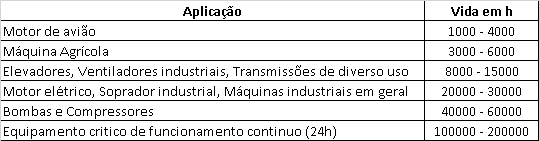
\includegraphics[scale=0.99]{Imagens/Img15.png}\\
    {\footnotesize Fonte: Adaptado de Mott (2013)}
    \label{fig:15}
\end{figure}


Outra forma de encontrar o fator de ciclagem de tensão para resistência
ao crateramento é ingressando o valor de ciclos desejado no gráfico da
Figura {\ref{fig:16}}.~A parte inferior da zona
sombreada, da Figura {\ref{fig:16}}, é normalmente
usada para serviços críticos, onde o desgaste por crateramento no dente
deve ser mínimo e são necessários baixos níveis de vibração.\selectlanguage{brazil}

\begin{figure}[!htb]
    \centering
    \caption{Fator de ciclagem de tensão para a resistência ao crateramento}
    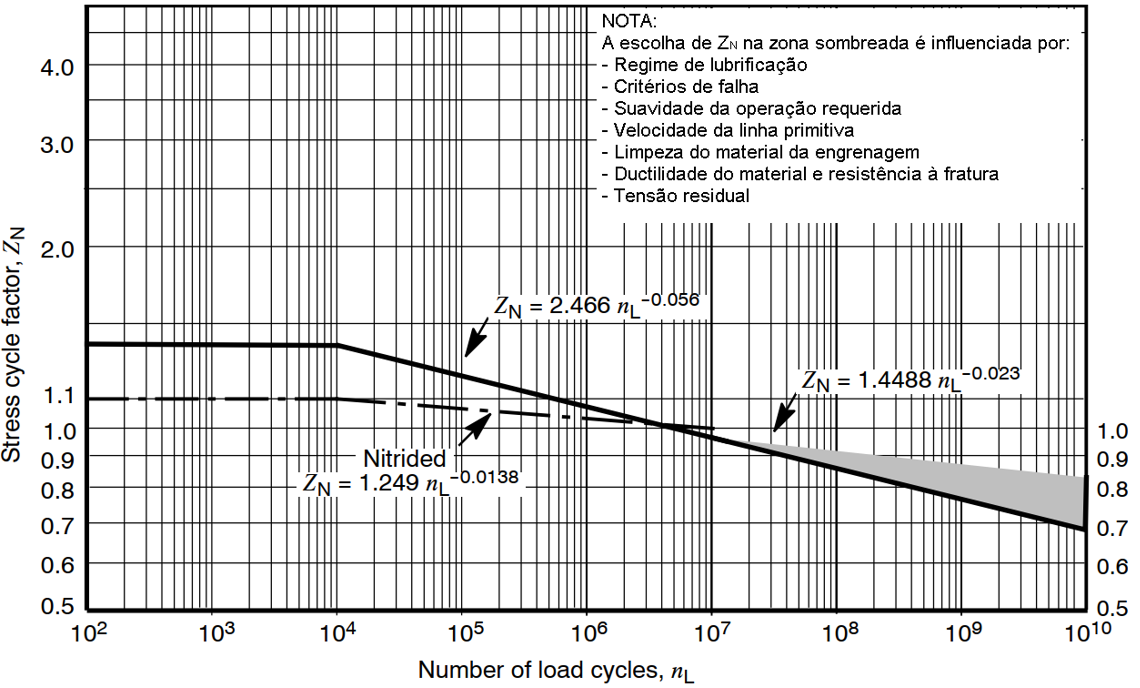
\includegraphics[scale=0.5]{Imagens/Img16.png}\\
    {\footnotesize Fonte: Adaptado de ANSI/AGMA 2101-D04 (2016)}
    \label{fig:16}
\end{figure}

\subsubsection*{\texorpdfstring{Fator de razão de dureza,
Z\textsubscript{W}}{Fator de razão de dureza, ZW}}

{\label{fator-de-razuxe3o-de-dureza-zw}}

O fator de razão de dureza, \emph{Z}\textsubscript{W}, depende de:

\begin{itemize}
\tightlist
\item
  A relação de transmissão;
\item
  O acabamento superficial no flanco do dente do pinhão;
\item
  A dureza na superfície das engrenagens (pinhão e coroa).
\end{itemize}

O valor de \emph{Z}\textsubscript{W} para o pinhão é fixado em 1,0. Já o
valor de \emph{Z}\textsubscript{W} para a coroa é 1.0 ou conforme
descrito a seguir.

\subsubsection*{Coroas endurecidas}

{\label{coroas-endurecidas}}

Quando a superfície do pinhão é substancialmente mais dura do que a
superfície da coroa, durante o engrenamento o pinhão endurece a coroa.
Os valores típicos de~\emph{Z}\textsubscript{W} para coroas, nesse
cenário, pode ser calculado com a Equação {\ref{eq21}}.

\par\null

\begin{equation}
\label{eq21}
Z_{\mathrm{W}}\mathrm{=1,0+}A\left(i\mathrm{-}\mathrm{1,0}\right)
\end{equation}

\par\null

Se \(\frac{H_{B1}}{H_{B2}}<1,2\ \rightarrow A=0\)

Se\(1,2\leq\frac{H_{B1}}{H_{B2}}\leq 1,7\ \rightarrow A=0,00898\left(\frac{H_{B1}}{H_{B2}}\right)-0,00829\)

Se \(\frac{H_{B1}}{H_{B2}}>1,7\ \rightarrow A=0,00698\)

Onde

\(H_{B1}\) é a dureza Brinell do pinhão, HB;

\(H_{B2}\) é a dureza Brinell da coroa, HB;

\(i\) é a relação de velocidade entre engrenagens.

Também, o fator de dureza de superfície pode ser encontrado com o
gráfico apresentado na Figura {\ref{fig:17}}.\selectlanguage{brazil}

\begin{figure}[!htb]
    \centering
    \caption{Fator de relação de dureza}
    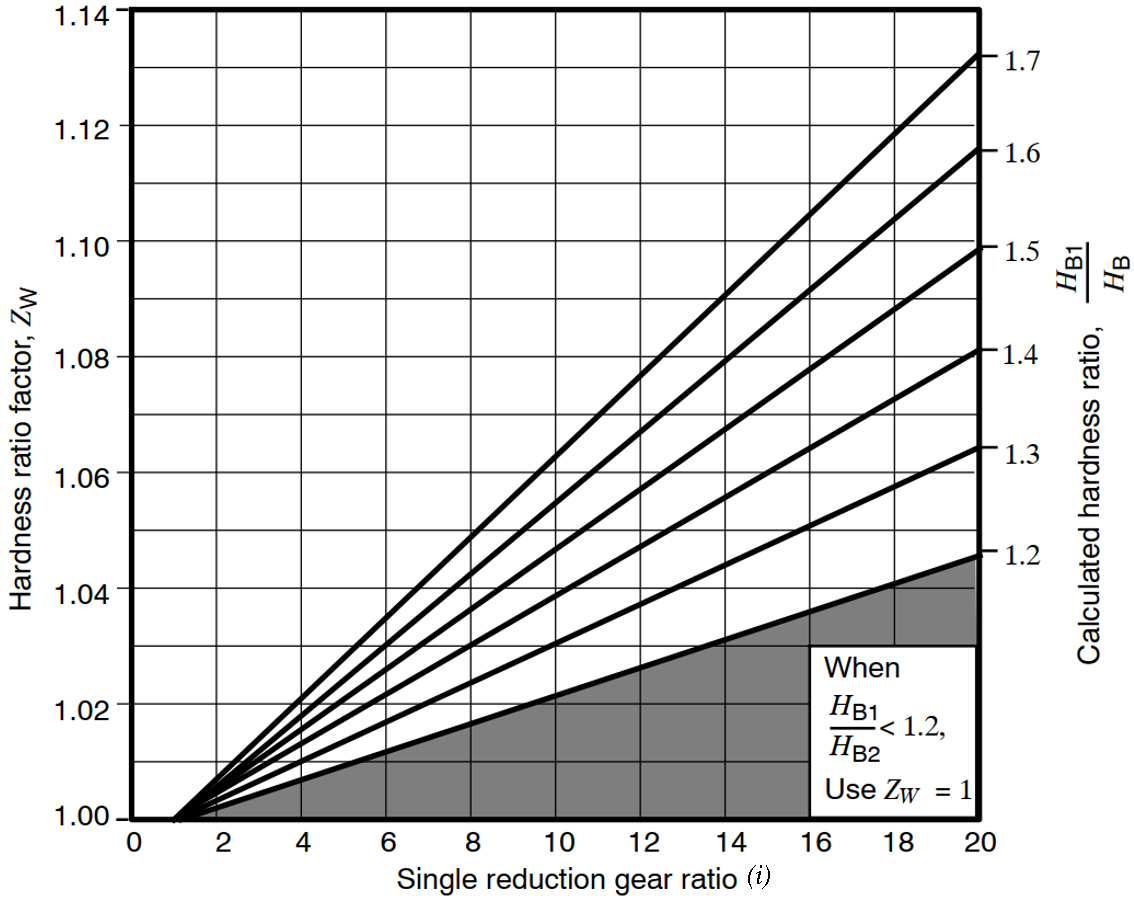
\includegraphics[scale=0.5]{Imagens/Img17.png}\\
    {\footnotesize Fonte: Adaptado de ANSI/AGMA 2101-D04 (2016)}
    \label{fig:17}
\end{figure}

\subsubsection*{Endurecido superficial/através de valores
endurecidos}

{\label{endurecido-superficialatravuxe9s-de-valores-endurecidos}}

Quando a superfície do pinhão endurecida (de 460 HB ou mais) engrena com
uma coroa endurecida (entre 180 HB a 400 HB), o
fator~\emph{Z}\textsubscript{W} varia com o acabamento da superfície do
pinhão, dependendo da sua altura máxima do perfil de rugosidade do
pinhão (\emph{R}\textsubscript{z1}). A dureza da coroa correspondente
pode ser obtida com a Equação {\ref{eq22}}.

\par\null

\begin{equation}
\label{eq22}
Z_{\mathrm{W}}\mathrm{=1,0+}B\left(\mathrm{450-}H_{\mathrm{B2}}\right)
\end{equation}

\par\null

Onde

B = 0,00075 (\emph{e} )\textsuperscript{-0,448(\emph{Rz}1)}

\emph{e} é a base dos logaritmos naturais ou napierianos = 2,718 28

\emph{R}\textsubscript{Z1} é o acabamento superficial final do pinhão,$\mu$m.

Esse valor de \emph{Z}\textsubscript{W} também pode ser obtido do
gráfico da Figura {\ref{fig:18}}.\selectlanguage{brazil}

\begin{figure}[!htb]
    \centering
    \caption{Fator de relação de dureza}
    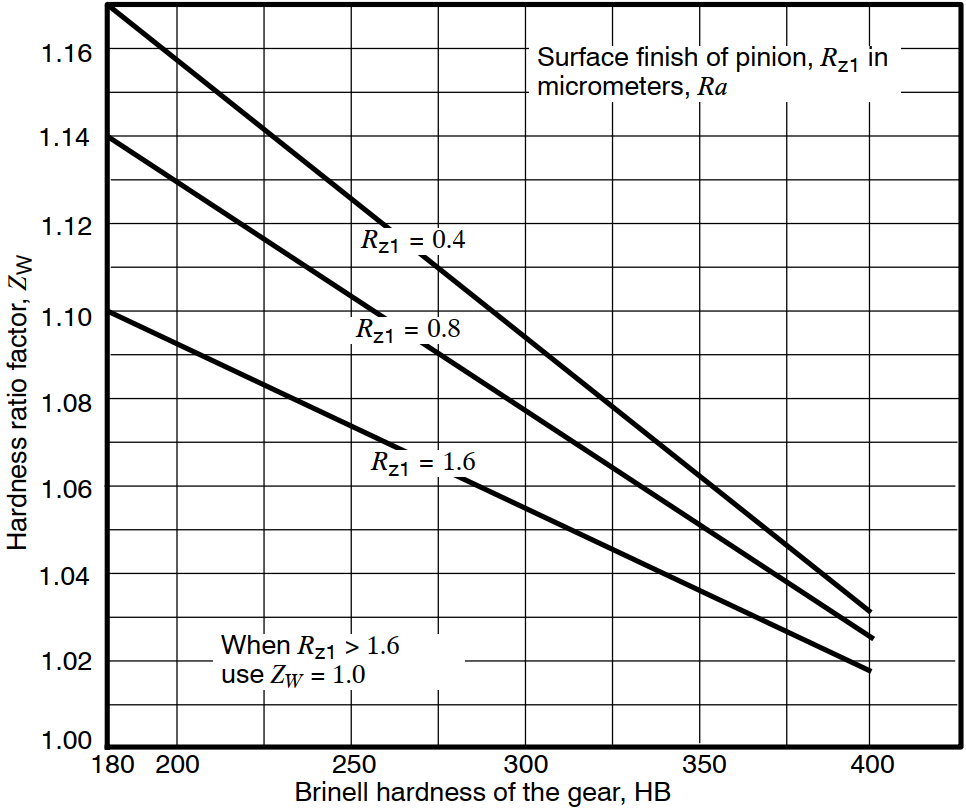
\includegraphics[scale=0.5]{Imagens/Img18.png}\\
    {\footnotesize Fonte: Adaptado de ANSI/AGMA 2101-D04 (2016)}
    \label{fig:18}
\end{figure}

\subsubsection*{\texorpdfstring{Fator de
confiabilidade,~\emph{Y}\textsubscript{Z}}{Fator de confiabilidade,~YZ}}

{\label{fator-de-confiabilidade-yz}}

O fator de confiabilidade é responsável pelo efeito da distribuição
estatística normal das falhas encontradas nos testes de materiais usados
para engrenagens. Os números de tensão permitidos apresentados na norma
são baseados na probabilidade estatística de 01 falha em 100 a
10\textsuperscript{7} ciclos. A Tabela~{\ref{tab:2}}
contém fatores de confiabilidade que podem ser usados para modificar
essas tensões permitidas para alterar essa probabilidade. Esses números
são baseados em dados desenvolvidos pela Marinha dos EUA.\selectlanguage{brazil}

\begin{table}[!htb]
\centering
\caption{{\label{tab:2} Fator de confiabilidade pelo número de falhas}}
\begin{tabular}{ l c c}
\hline
\textbf{Requisitos de aplicação}        &\textbf{$Y_Z \ ^{1)}$} \\ \hline
Menos de uma falha em 10 000            & 1,5       \\
Menos de uma falha em 1000              & 1,25      \\
Menos de uma falha em 100               & 1,0       \\
Menos de uma falha em 10                & $0,85\ ^{2)}$   \\
Menos de uma falha em 2                 & $0,7\ ^{2) 3)}$ \\
\hline
\end{tabular}
\end{table}

Nota:

1) às vezes, a quebra por flexão, no dente, é considerada um risco maior
do que por crateramento. Nesses casos, um valor maior
de~\emph{Y}\textsubscript{Z} é selecionado para flexão.

2) nesse valor, pode ocorrer um fluxo plástico ao invés de crateramento.

3) fruto da extrapolação dos dados de teste.

Para~\hyperref[csl:20]{(Budynas \& Nisbett, 2014)} o fator de confiabilidade também pode ser obtido
conforme apresentado na Figura {\ref{fig:19}}.\selectlanguage{brazil}

\begin{figure}[!htb]
    \centering
    \caption{Fator de confiabilidade: falhas por fadiga do material}
    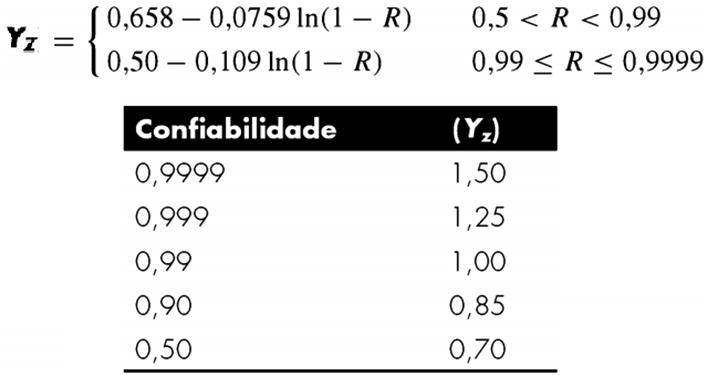
\includegraphics[scale=0.5]{Imagens/Img19.png}\\
    {\footnotesize Fonte: Adaptado de Buday e Nisbett (2014)}
    \label{fig:19}
\end{figure}

\subsubsection*{Fator de
temperatura,~\(Y_{\mathbf{\theta}}\)}

{\label{fator-de-temperatura-yux3b8}}

O fator de temperatura é geralmente 1,0 quando as próprias engrenagens
ou a temperatura de óleo lubrificante opera com temperatura não
superiores a 120 °C. Quando as temperaturas de operação é abaixo de 0 °
C, deve-se ter cuidado especial.

Quando a temperatura do óleo ou da engrenagem opera acima de 120 °C, é
atribuído ao fator de temperatura um valor maior que 1,0 mas, e
isso depende da experiência do engenheiro projetista.

Na análise envolvendo a temperatura de trabalho, deve-se considerar a
perda de dureza e consequente resistência ao crateramento, de alguns
materiais quando operando a temperaturas acima de 150 ° C.

\subsubsection*{Número de tensão ao contato
permitida,~\(\mathbf{\sigma}_{\mathbf{\text{HP}}}\)}

{\label{nuxfamero-de-tensuxe3o-ao-contato-permitida-mathbfsigma_mathbftexthp}}

Os números de tensão permitidos para materiais de engrenagem variam de
acordo com fatores como: a composição do material, limpeza durante a
têmpera, tensão residual, microestrutura, qualidade do processo de
manufatura, tipo tratamento térmico e práticas de processamento. Para
outros materiais diferentes do aço, é exibida uma faixa e, os valores
mais baixos devem ser usados para fins gerais de projeto. Para aço deve
ser usada a Figura~{\ref{fig:20}}.\selectlanguage{brazil}

\begin{figure}[!htb]
    \centering
    \caption{Número de tensão permitida ao contato, para aço}
    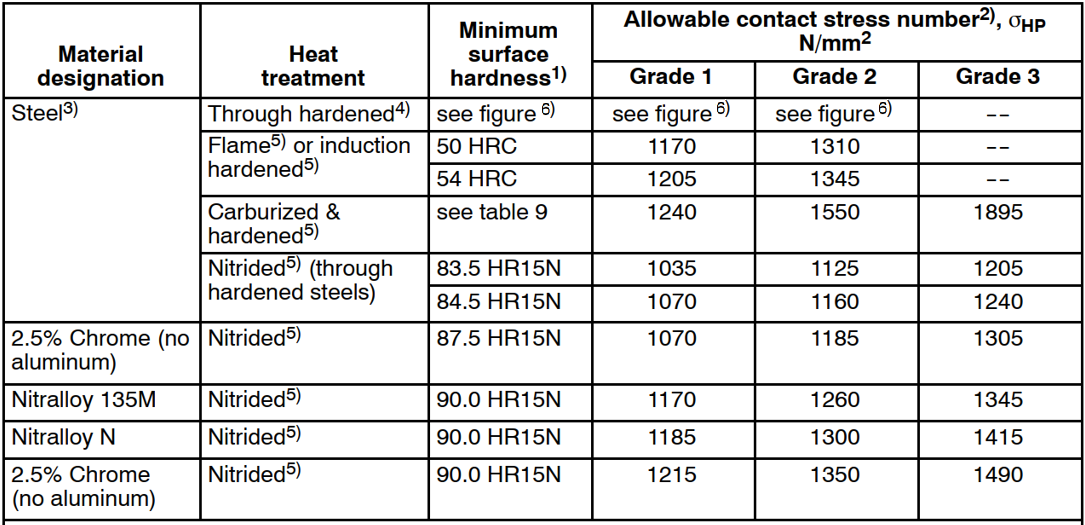
\includegraphics[scale=0.55]{Imagens/Img20.png}\\
    {\footnotesize Fonte: Adaptado de ANSI/AGMA 2101-D04 (2016)}
    \label{fig:20}
\end{figure}

NOTAS da Figura \ref{fig:20}:

1) Dureza no início do centro da largura da face do dente.

2) Consulte a norma AGMA 2101-D04 para verificar fatores metalúrgicos
que afetam o número de tensão de contato
permitido,$\sigma_{HP}$, nas engrenagens de aço.

3) O aço selecionado deve ser compatível com o processo de tratamento
térmico selecionado e a dureza necessária.

4) O material deve ser revenido, recozido ou no mínimo normalizado.

5) O $\sigma_{HP}$ no dente da engrenagem endurecida na
superfície, requerem de uma profundidade adequada para resistir às
tensões de cisalhamento desenvolvidas pelas cargas de contato do dente e
pelas tensões de tração do cordão raiz do dente, mas, a profundidade não
deve ser tão grande que resulte em pontas de dentes quebradiças e com
altas tensões de tração residual no núcleo.

6) ver gráfico da Figura~{\ref{fig:21}}.

Outra forma de encontrar a dureza, adequada para a superfície do dente é
por meio da Figura~{\ref{fig:21}}.\selectlanguage{brazil}

\begin{figure}[!htb]
    \centering
    \caption{Número de tensão permitida ao contato, para aço}
    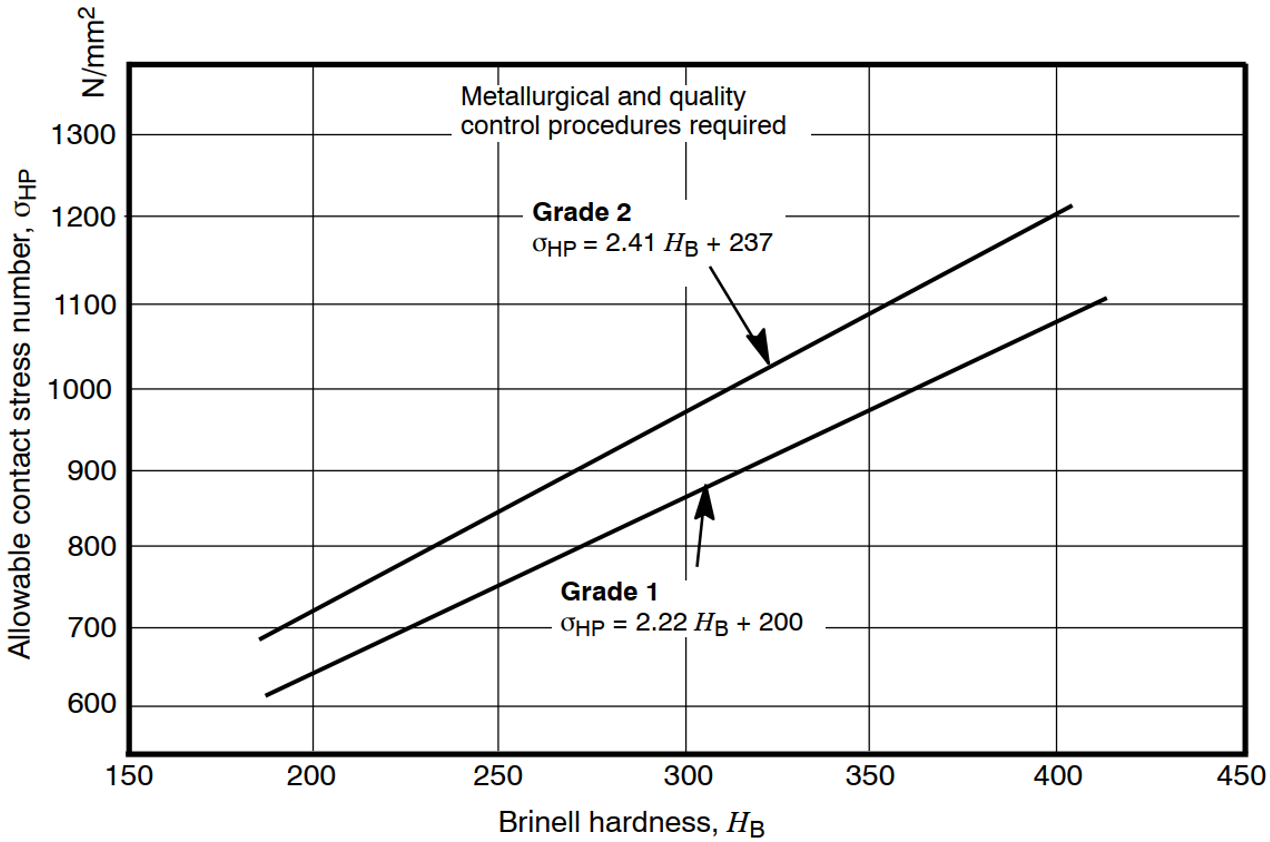
\includegraphics[scale=0.45]{Imagens/Img21.png}\\
    {\footnotesize Fonte: Adaptado de ANSI/AGMA 2101-D04 (2016)}
    \label{fig:21}
\end{figure}

\par\null

Segundo a AGMA 2101-D04 (2016), para determinar a profundidade do
endurecimento no dente, depende do módulo usado, a maior módulo maior a
profundidade de endurecimento, podendo variar de 1,2 até 5,2 mm de
profundidade, aproximadamente.

Na Figura {\ref{fig:22}}, pode ser observada a variação
nos processos para obter endurecimento nos dentes da engrenagem, quando
aplicados endurecimento por chama ou indução: girando a engrenagem para
seu endurecimento, endurecimento somente no flanco (dente a dente), e
endurecimento de flanco e raiz (dente a dente).\selectlanguage{brazil}

\begin{figure}[!htb]
    \centering
    \caption{Processos para endurecimento por chama ou indução}
    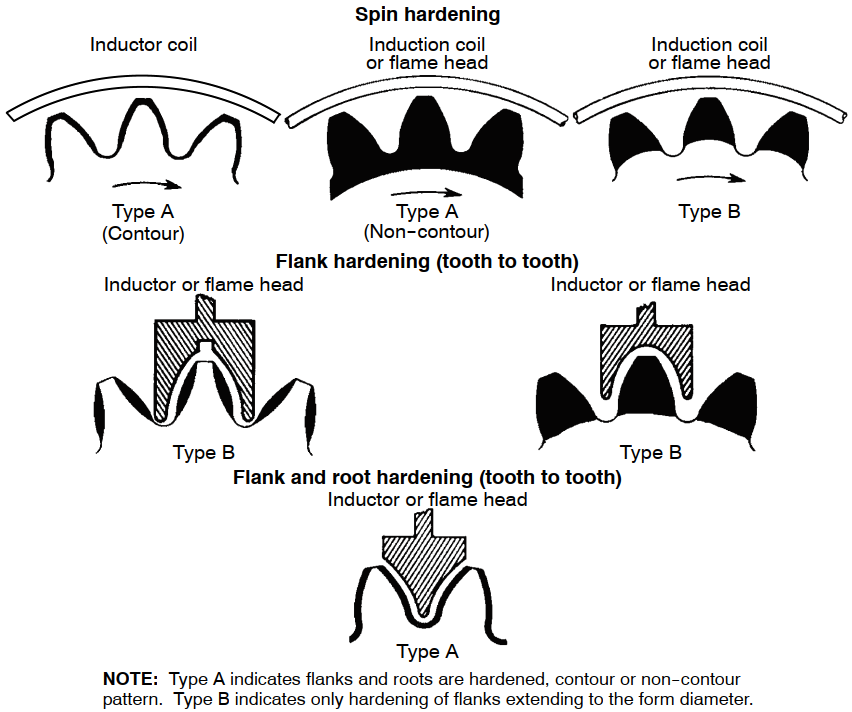
\includegraphics[scale=0.45]{Imagens/Img22.png}\\
    {\footnotesize Fonte: Adaptado de ANSI/AGMA 2101-D04 (2016)}
    \label{fig:22}
\end{figure}

Para encontrar o $\sigma_{\text{HP}}$ para engrenagens que não sejam de aço, pode ser usada a Figura {\ref{fig:23}}.\selectlanguage{brazil}

\begin{figure}[!htb]
    \centering
    \caption{Número de tensão permitida ao contato, para ferro fundido e bronze}
    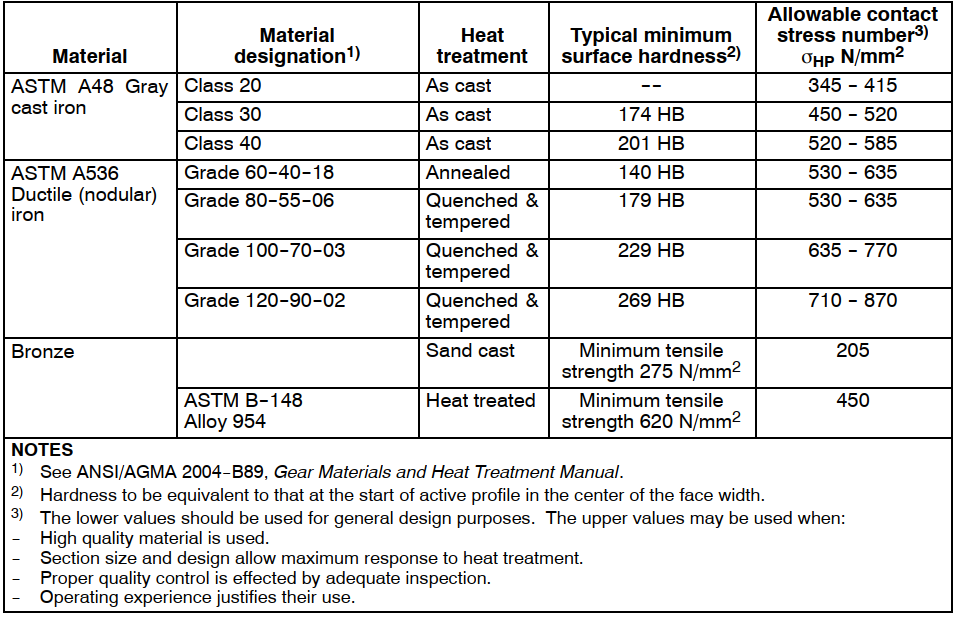
\includegraphics[scale=0.6]{Imagens/Img23.png}\\
    {\footnotesize Fonte: Adaptado de ANSI/AGMA 2101-D04 (2016)}
    \label{fig:23}
\end{figure}

\subsection*{Resistência à Flexão}

{\label{resistencia-uxe0-flexuxe3o}}

A resistência à flexão nos dentes de uma engrenagem é um fenômeno de
fadiga relacionado à resistência à fratura na região do cordão raiz do
dente da engrenagem.

\subsection*{Tensão à Flexão
AGMA,~\(\mathbf{\sigma}_{\mathbf{F}}\)}

{\label{tensuxe3o-uxe0-flexuxe3o-agma-mathbfsigma_mathbff}}

Para calcular a tensão à flexão, todas as definições a seguir serão
usando a norma ANSI/AGMA \hyperref[csl:5]{(2101-D04, 2016)}. A maioria dos fatores da
Equação {\ref{eq23}} para tensão à flexão já foram
abordadas no item Tensão ao contato AGMA.

\par\null

\begin{equation}
\label{eq23}
{\sigma }_F\mathrm{=}\frac{W^t\mathrm{\cdot }K_{\mathrm{O}}\mathrm{\cdot }K_{\mathrm{V}}\mathrm{\cdot }K_{\mathrm{S}}\mathrm{\cdot }K_{\mathrm{H}}\mathrm{\cdot }K_{\mathrm{B}}}{b\mathrm{\cdot }m_n\mathrm{\cdot }Y_{\mathrm{J}}}
\end{equation}



Onde

\(\sigma_{F}\) è a tensão à flexão, N/mm\textsuperscript{2};

\(W^{t}\) é a carga tangencial transmitida, N;

\(K_{O}\) é o fator de sobrecarga;

\(K_{V}\) é o fator dinâmico;

\(K_{S}\) é o fator de tamanho;

\(K_{H}\) é o fator de distribuição de carga;

\(K_{B}\) é o fator de espessura de borda;

\(b\) é a largura da face da engrenagem mais estreita, mm;

\(m_{n}\) é o módulo métrico normal, mm;

\(Y_{J}\) é o fator geométrico para resistência à flexão
(inclui o fator de concentração de tensão do cordão raiz
\(K_{f}\)).

\subsubsection*{\texorpdfstring{Fator de espessura de
borda,~\emph{K}\textsubscript{B}}{Fator de espessura de borda,~KB}}

{\label{fator-de-espessura-de-borda-kb}}

Quando a espessura da borda não é suficiente para fornecer um suporte
total ao cordão raiz do dente, o local de falha por fadiga à flexão pode
ser na borda da engrenagem, e não no filete do cordão raiz. O fator de
espessura de borda, \emph{K}\textsubscript{B}, não é suficientemente
conservador para tensões com furos na alma (ou nervura) e, rasgos de
chaveta ou entalhes no cubo.

O \emph{K}\textsubscript{B} ajusta o valor do cálculo para a tensão à
flexão nas engrenagens com borda estreita. Para tal, deve ser encontrada
primeiro a relação de espessura da borda abaixo do cordão raiz do
dente,~\emph{m}\textsubscript{B}, conforme Equação
{\ref{eq24}}.

\par\null

\begin{equation}
\label{eq24}
m_{\mathrm{B}}\mathrm{=}\frac{t_{\mathrm{R}}}{h_{\mathrm{t}}}
\end{equation}

\par\null

Onde

\emph{t}\textsubscript{R} é a espessura da borda abaixo da raiz do
dente, mm;

\emph{h}\textsubscript{t} é altura total do dente, mm.

Dependendo do valor obtido, se for maior ou igual a 1,2 o fator de borda
sempre será 1,0. Se o valor obtido for menor do que 1,2 deve ser usada a
equação contida na Figura {\ref{fig:24}}.\selectlanguage{brazil}

\begin{figure}[!htb]
    \centering
    \caption{Características do fator de borda}
    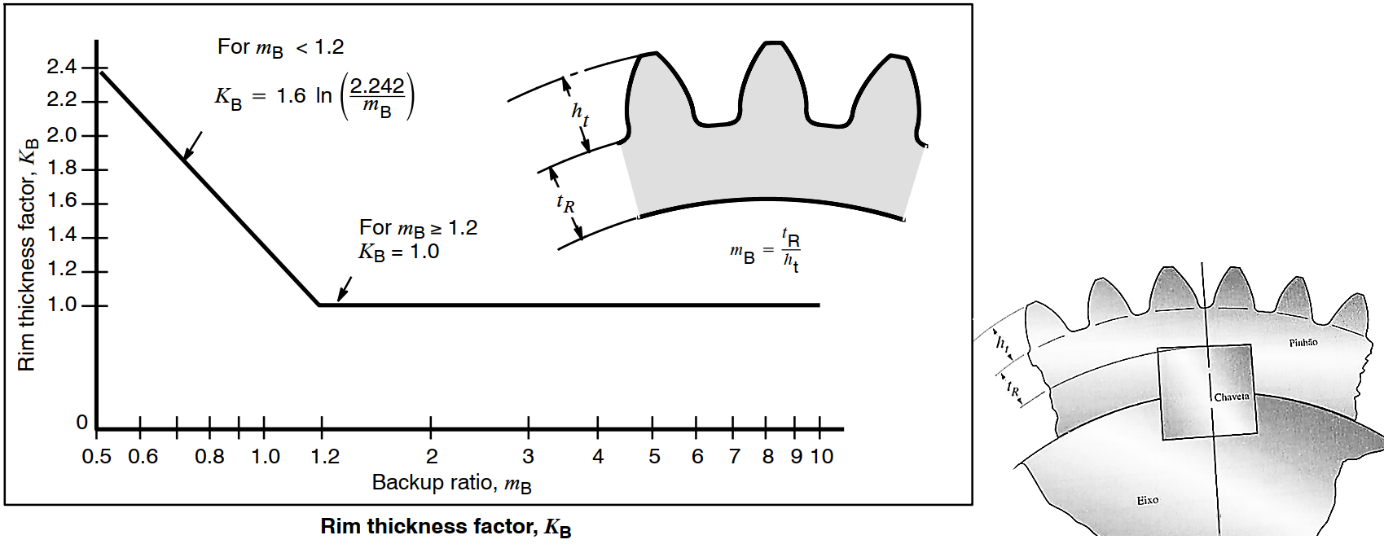
\includegraphics[scale=0.9]{Imagens/Img24.png}\\
    {\footnotesize Fonte: Adaptado de Mott (2013)}
    \label{fig:24}
\end{figure}

\subsubsection*{\texorpdfstring{Fator de geometria,~\emph{Y}\textsubscript{J}}{Fator de geometria,~YJ}}

{\label{fator-de-geometria-yj}}

O fator de geometria avalia o raio do cordão raiz da involuta do dente,
e leva em consideração o fator de forma de Lewis modificado e a sus
distribuição da carga.

O fator de geometria é determinado pela norma AGMA 908 - B89 confirmada
em 2015, além disso, estudos recentes também confirmam a aplicabilidade
da norma AGMA para encontrar o fator geométrico \hyperref[csl:26]{(Frechilla et al., 2016)}.

A AGMA inclui tabelas para algumas formas comuns de dentes e o método
analítico para involuta de engrenagens com cordão de raiz gerados. O
fator de geometria, \emph{Y}\textsubscript{J}, é um valor sem dimensão,
e leva em consideração os efeitos de:

\begin{itemize}
\tightlist
\item
  Forma do dente;
\item
  Pior posição de carga;
\item
  Concentração de tensão;
\end{itemize}

Nesse fator de geometria estão incluídas as cargas no dente tanto no
componente tangencial como no componente radial. Esta análise se aplica
apenas a engrenagens externas.

Uma forma rápida de encontrar o \emph{Y}\textsubscript{J} é usando a
Figura {\ref{fig:25}} que considera um cordão raiz
produto da multiplicação do módulo vezes a constante 0,35. O gráfico
deve ser usado apenas para engrenagem com ângulo de pressão (ou contato)
igual a 20° \hyperref[csl:20]{(Budynas \& Nisbett, 2014}; \hyperref[csl:21]{Mott, 2013}; \hyperref[csl:27]{Juvinall \& Marshek, 2011)}.\selectlanguage{Brazil}

\begin{figure}[!htb]
    \centering
    \caption{Fator geométrico para engrenagem com ângulo de pressão 20°}
    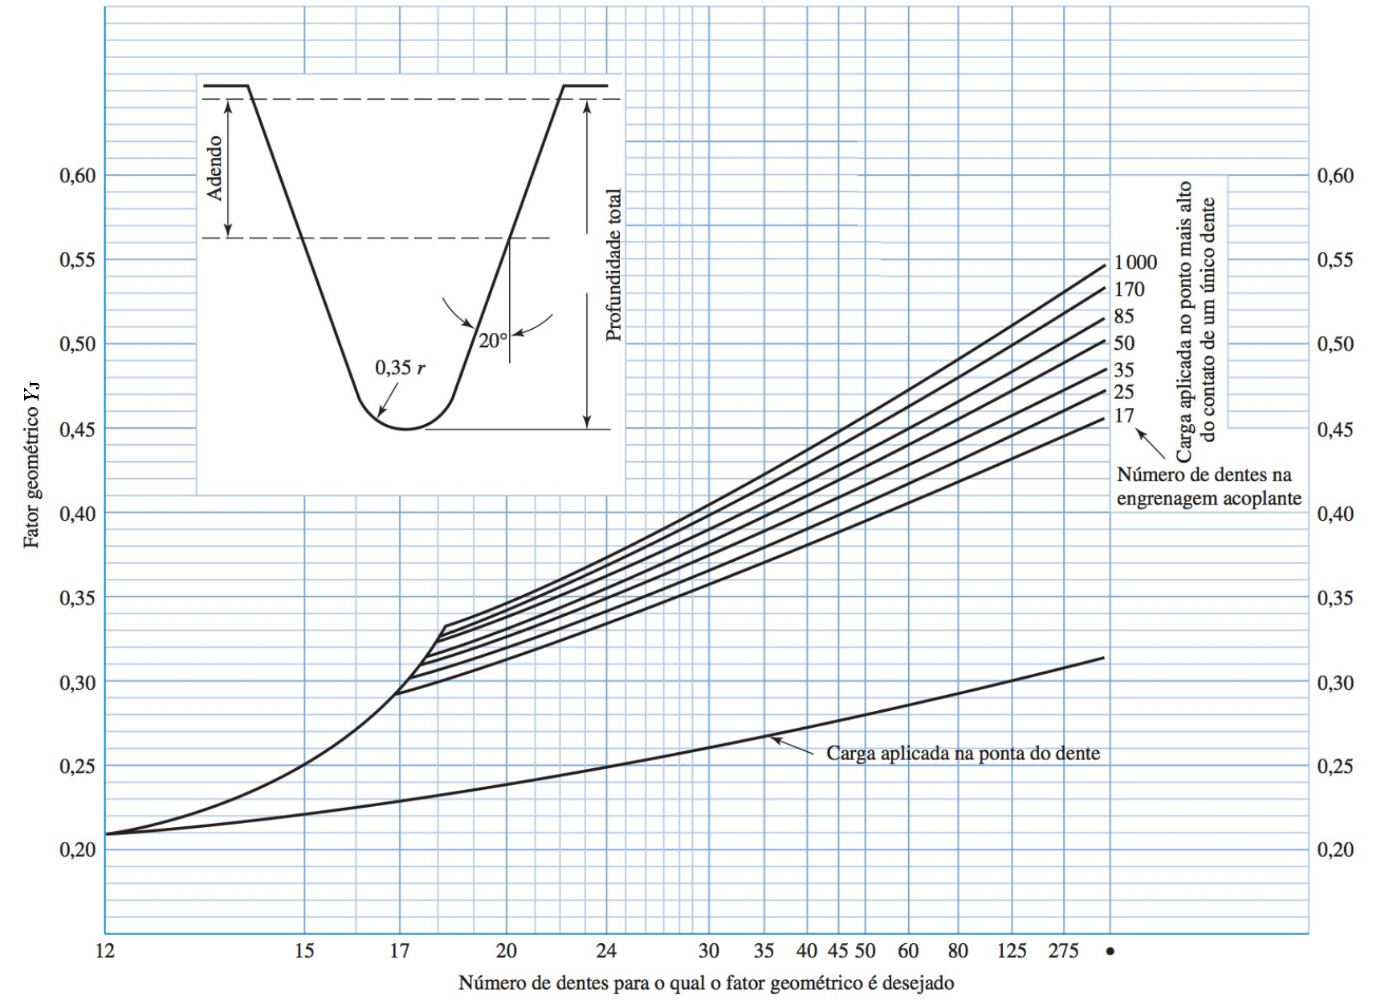
\includegraphics[scale=0.99]{Imagens/Img25.png}\\
    {\footnotesize Fonte: Adaptado Buday e Nisbett (2014)}
    \label{fig:25}
\end{figure}

\subsection*{\texorpdfstring{Fator de segurança AGMA à
flexão,~\emph{S}\textsubscript{F}}{Fator de segurança AGMA à flexão,~SF}}

{\label{fator-de-seguranuxe7a-agma-uxe0-flexuxe3o-sf}}

Para o fator de segurança AGMA à flexão recomenda-se que esse valor
esteja no intervalo de 1 a 1,5~\hyperref[csl:21]{(Mott, 2013)}. A
Equação~{\ref{eq25}} serve para encontrar esse fator de
segurança que garante uma resistência à flexão de projeto, lembrando que
a tensão à flexão, $\sigma_{\text{F}}$, já foi abordada.

\par\null

\begin{equation}
\label{eq25}
S_{\mathrm{F}}\mathrm{=}\frac{{\sigma }_{\mathrm{FP}}}{{\sigma }_{\mathrm{F}}}\cdot \frac{Y_{\mathrm{N}}}{Y_{\mathrm{\theta }}\cdot Y_{\mathrm{Z}}}
\end{equation}

\par\null

Onde

\(S_{F}\) é o fator de segurança AGMA à flexão;

\(\sigma_{\text{FP}}\) é o número de tensão à flexão permitida
AGMA,\(\frac{N}{\text{mm}^{2}}\);

\(\sigma_{F}\) é a tensão à flexão AGMA, \(\frac{N}{\text{mm}^{2}}.\)

\(Y_{N}\) é o fator de ciclagem para resistência à flexão;

\(Y_{Z}\) é o fator de confiabilidade;

\(Y_{\theta}\) é o fator de temperatura.

A maioria dos fatores para encontrar o fator de segurança AGMA à flexão
já foram detalhados anteriormente. Nesta seção serão abordados apenas o
fator de ciclagem,~\emph{Y}\textsubscript{N}, e o número de tensão à
flexão permitido $\sigma_{\text{FP}}$. Cabe destacar que $\sigma_{\text{FP}}$ não tem relação
com~\emph{S}~\textsubscript{y}\emph{,
S}~\textsubscript{ut},~\emph{S}~\textsubscript{e}'
ou~\emph{S}~\textsubscript{e}, deve ser usado apenas para fator de
segurança AGMA.

\subsubsection*{\texorpdfstring{Fator de ciclagem de tensão à
flexão,~\emph{Y}\textsubscript{N}}{Fator de ciclagem de tensão à flexão,~YN}}

{\label{fator-de-ciclagem-de-tensuxe3o-uxe0-flexuxe3o-yn}}

Atualmente, não há dados suficientes para fornecer gráficos precisos de
ciclagem de tensão para todos os tipos de engrenagens e suas aplicações.
A experiência, no entanto, sugere valores do ciclo de tensão para
resistência à flexão de engrenagens de aço, como mostrado na Figuras
{\ref{fig:26}}. Esse gráfico termina em
10\textsuperscript{10} ciclos, devido a dados insuficientes no momento
em que foi elaborada a norma. Esse gráfico não deve ser usado para
engrenagens de aço inoxidável. A zona sombreada na imagem representa a
influência com a velocidade linear, limpeza do material, qualidade no
processo de manufatura boa, ductilidade do material e resistência à
fratura.\selectlanguage{brazil}

\begin{figure}[!htb]
    \centering
    \caption{Fator de ciclagem a flexão para aço}
    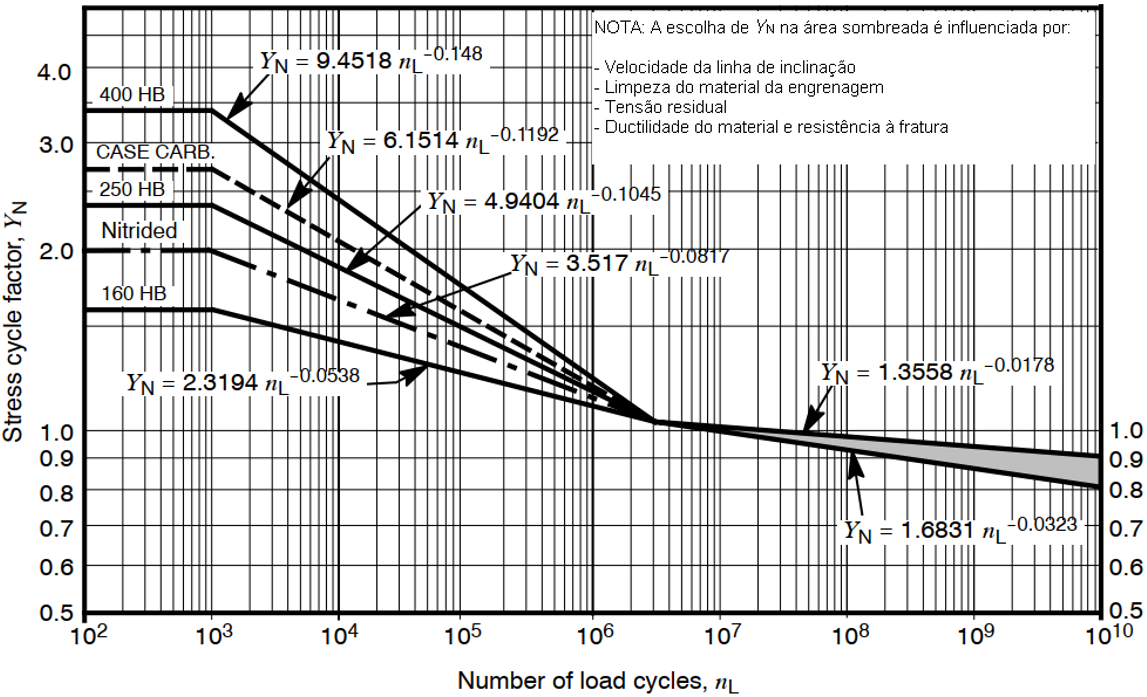
\includegraphics[scale=0.5]{Imagens/Img26.png}\\
    {\footnotesize Fonte: Adaptado de ANSI/AGMA 2101-D04 (2016)}
    \label{fig:26}
\end{figure}


Para \hyperref[csl:21]{(Mott, 2013)}, a parte superior da zona sombreada é para
aplicações gerais e recomendada para projetos de engrenagens, assim,
pode ser usada a Equação {\ref{eq26}}.

\par\null

\begin{equation}
\label{eq26}
Y_{\mathrm{N}}\mathrm{=1,3558}\mathrm{\cdot }{n_{\mathrm{L}}}^{\mathrm{-}\mathrm{0,0178}}
\end{equation}

\par\null

Os valores intermediários de~\emph{Y}\textsubscript{N} de
10\textsuperscript{3} a 3 × 10\textsuperscript{6}, para durezas de
engrenagens, podem ser aproximados determinando primeiro o valor usando
a interpolação logarítmica apresentada na
Figura~{\ref{fig:26}},~ um ponto para a dureza
desejada, no gráfico, de 3 × 10 ciclos é~\emph{Y}\textsubscript{N} = 1,04.
Abaixo de 10\textsuperscript{3} ciclos, o valor é uma constante, e
também obtida da Figura {\ref{fig:26}}.

O fator de ciclagem de tensão, \emph{Y}\textsubscript{N}, ajusta o
número de tensão ao contato permitido para ciclos de operação
requeridos. Para os fins desta norma, \emph{n}\textsubscript{L}, é o
número de ciclos de tensão e é definido como o número de contatos de
engrenamento, sob carga, do dente da engrenagem sendo analisado. Os
números de tensão permitido pela AGMA são estabelecidos para
10\textsuperscript{7} ciclos de carga do dente unidirecional com 99\% de
confiabilidade.

O fator de ciclagem de tensão é responsável pelas características de
resistência a cada número de ciclos, (S -- N), do material da
engrenagem, bem como pelo aumento gradual da tensão do dente, que pode
ocorrer devido ao desgaste do dente, resultando em efeitos dinâmicos
aumentados e na distribuição de carga variável que pode ocorrer durante
o projeto da vida útil da engrenagem.

Ao avaliar as engrenagens, é importante saber quantos ciclos de tensão
experimentam durante a vida útil prevista do equipamento. Algumas
máquinas funcionam 24 horas por dia e operam por vinte ou mais anos.
Outras máquinas possuem engrenagens que possuem um ciclo de tensão
equivalente a algumas horas. O projetista de equipamentos deve projetar
o número de ciclos de tensão que são apropriados para cada aplicação.

\subsubsection*{Número de tensão à flexão
permitida,~\(\mathbf{\sigma}_{\mathbf{\text{FP}}}\)}

{\label{nuxfamero-de-tensuxe3o-uxe0-flexuxe3o-permitida-mathbfsigma_mathbftextfp}}

O número de tensão permitido para flexão, $\sigma_{\text{FP}}$, varia de acordo com a composição do
material, limpeza no processo de manufatura, tensão residual,
microestrutura, qualidade do processo e tratamento térmico. Sendo assim,
os valores mais baixos devem ser usados para fins gerais de projeto.

Os números de tensão permitidos para aço, da norma AGMA, podem ser
encontrados na Figura {\ref{fig:27}} e são determinados
ou estimados a partir de testes experimentais e experiências de campo
acumuladas. Esses valores são baseados no fator de sobrecarga de 10
milhões de ciclos de tensão (10\textsuperscript{7}), carga unidirecional
e confiabilidade nos testes de 99\%. O $\sigma_{\text{FP}}$ é ajustado pelo fator de ciclagem de tensão \emph{Y}\textsubscript{N}.\selectlanguage{brazil}

\begin{figure}[!htb]
    \centering
    \caption{Número de tensão à flexão permitida para aço}
    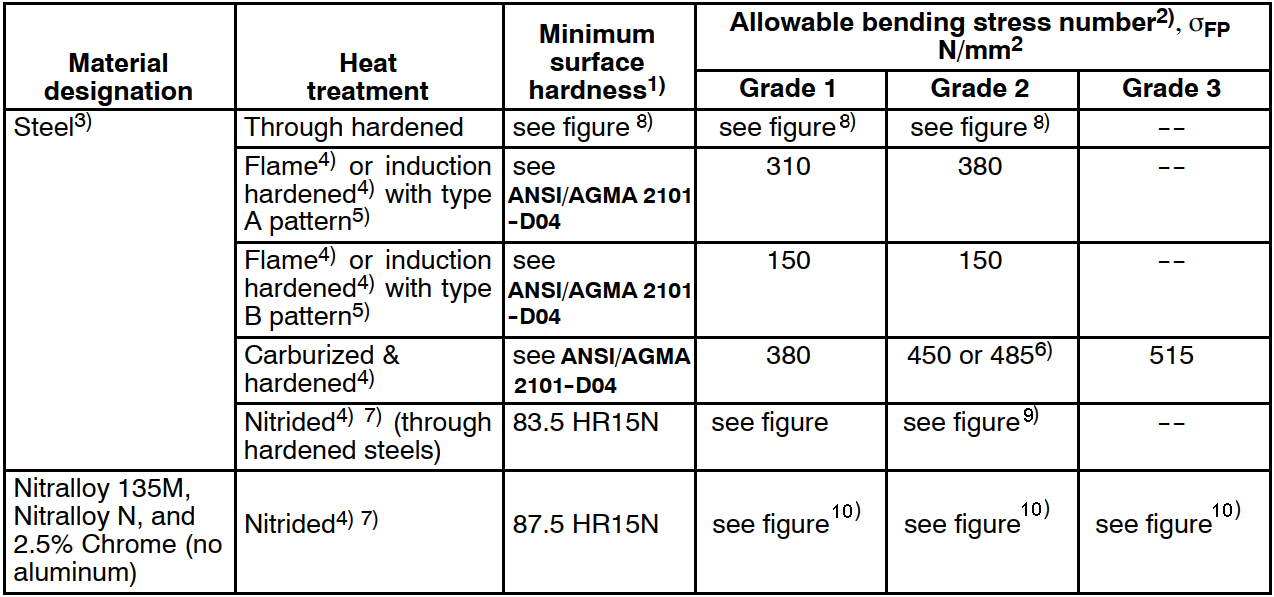
\includegraphics[scale=0.46]{Imagens/Img27.png}\\
    {\footnotesize Fonte: Adaptado de ANSI/AGMA 2101-D04 (2016)}
    \label{fig:27}
\end{figure}

NOTAS da Figura \ref{fig:27}:

1) Dureza equivalente no diâmetro raiz, no centro do espaço dos dentes e
da largura da face.

2) Veja a norma AGMA 2101-D04 para os principais fatores metalúrgicos de
cada grau de tensão.

3) O aço escolhido deve ser compatível com o processo de tratamento
térmico selecionado e a dureza requerida.

4) O número de tensão permitido indicado pode ser usado com as
profundidades de tempera prescritas na norma AGMA 2101-D04.

5) Veja a Figura~{\ref{fig:22}} para os padrões de
dureza do tipo A e tipo B.

6) Se a bainita e a microfissura estiverem limitadas aos níveis de Grau
3, pode ser usado 485 N/mm\textsuperscript{2}.

7) A capacidade de sobrecarga das engrenagens nitretadas é baixa. Como a
forma da curva S - N efetiva é plana, a sensibilidade ao choque deve ser
investigada antes de prosseguir com o projeto.

8) O número de tensão permitido a flexão pode ser obtido com o gráfico
da Figura~{\ref{fig:28}}.

9)~ O número de tensão permitido a flexão pode ser obtido com o gráfico
da Figura {\ref{fig:29}}.

10)~ O número de tensão permitido a flexão pode ser obtido com o gráfico
da Figura {\ref{fig:30}}.

Os números de tensão permitidos para as engrenagens de aço são
estabelecidos por requisitos específicos de controle de qualidade para
cada tipo e classe de material. Todos os requisitos para a nota de
qualidade devem ser atendidos para usar os valores de tensão dessa nota.
Isso pode ser conseguido certificando especificamente cada requisito,
quando necessário, ou estabelecendo práticas e procedimentos para obter
os requisitos em uma base de produção. Os valores intermediários não são
classificados, pois o efeito do desvio dos padrões de qualidade não pode
ser avaliado facilmente. Quando justificado por teste ou experiência,
níveis mais altos de tensão para qualquer série podem ser usados.\selectlanguage{brazil}

\begin{figure}[!htb]
    \centering
    \caption{Numero de tensão à flexão permitida para engrenagem de aço endurecida}
    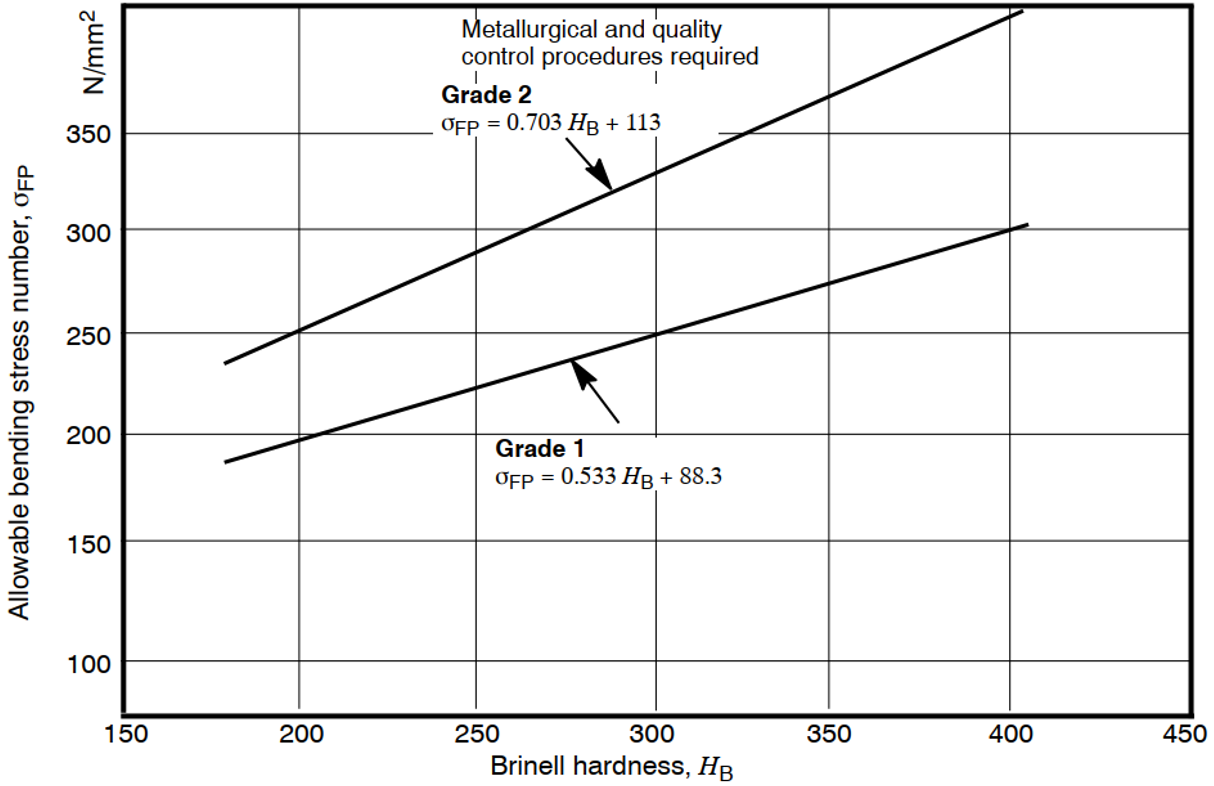
\includegraphics[scale=0.46]{Imagens/Img28.png}\\
    {\footnotesize Fonte: Adaptado de ANSI/AGMA 2101-D04 (2016)}
    \label{fig:28}
\end{figure}

\begin{figure}[!htb]
    \centering
    \caption{Numero de tensão à flexão permitida para nitretação de aço (AISI 4140 3 4340)}
    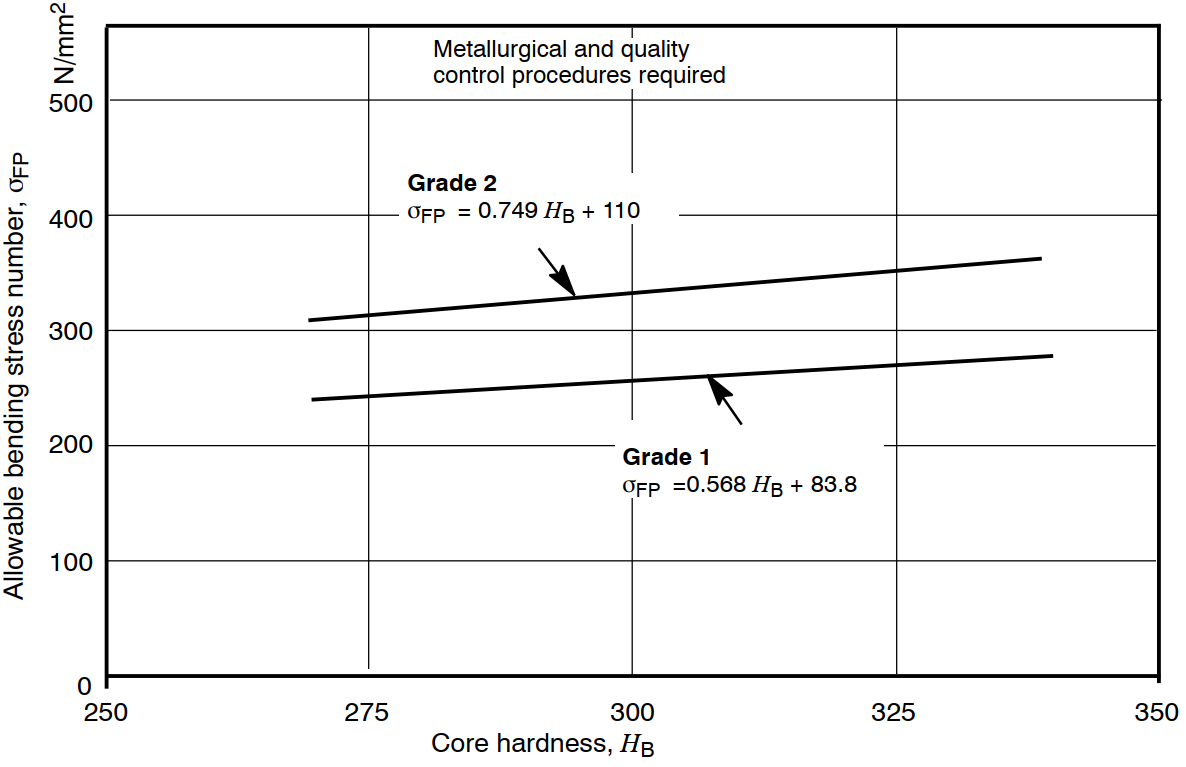
\includegraphics[scale=0.46]{Imagens/Img29.png}\\
    {\footnotesize Fonte: Adaptado de ANSI/AGMA 2101-D04 (2016)}
    \label{fig:29}
\end{figure}

\begin{figure}[!htb]
    \centering
    \caption{Numero de tensão à flexão permitida para nitretação de aços}
    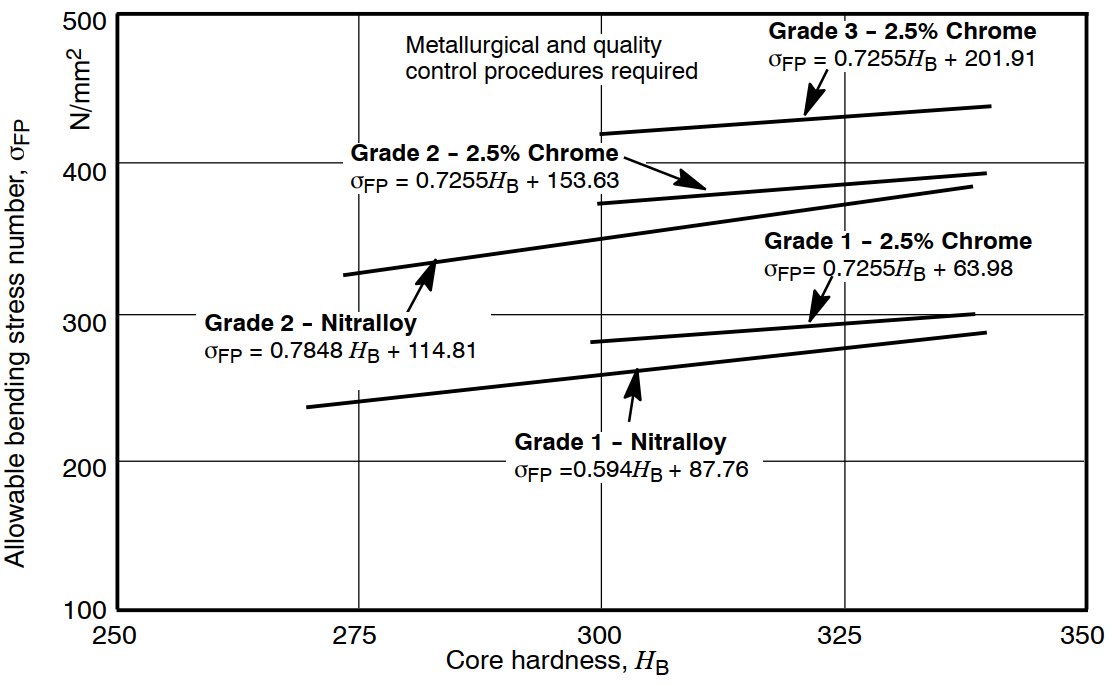
\includegraphics[scale=0.46]{Imagens/Img30.png}\\
    {\footnotesize Fonte: Adaptado de ANSI/AGMA 2101-D04 (2016)}
    \label{fig:30}
\end{figure}

Para os números de tensão permitidos para ferro e bronze nesta norma,
Figura {\ref{fig:31}}, também são determinados ou
estimados a partir de testes experimentais e experiências de campo
acumuladas. Eles são baseados no fator de sobrecarga de 10 milhões de
ciclos de tensão (10\textsuperscript{7}), carga unidirecional e
confiabilidade nos testes de 99\%.\selectlanguage{brazil}

\begin{figure}[!htb]
    \centering
    \caption{Numero de tensão à flexão permitida para ferro e bronze}
    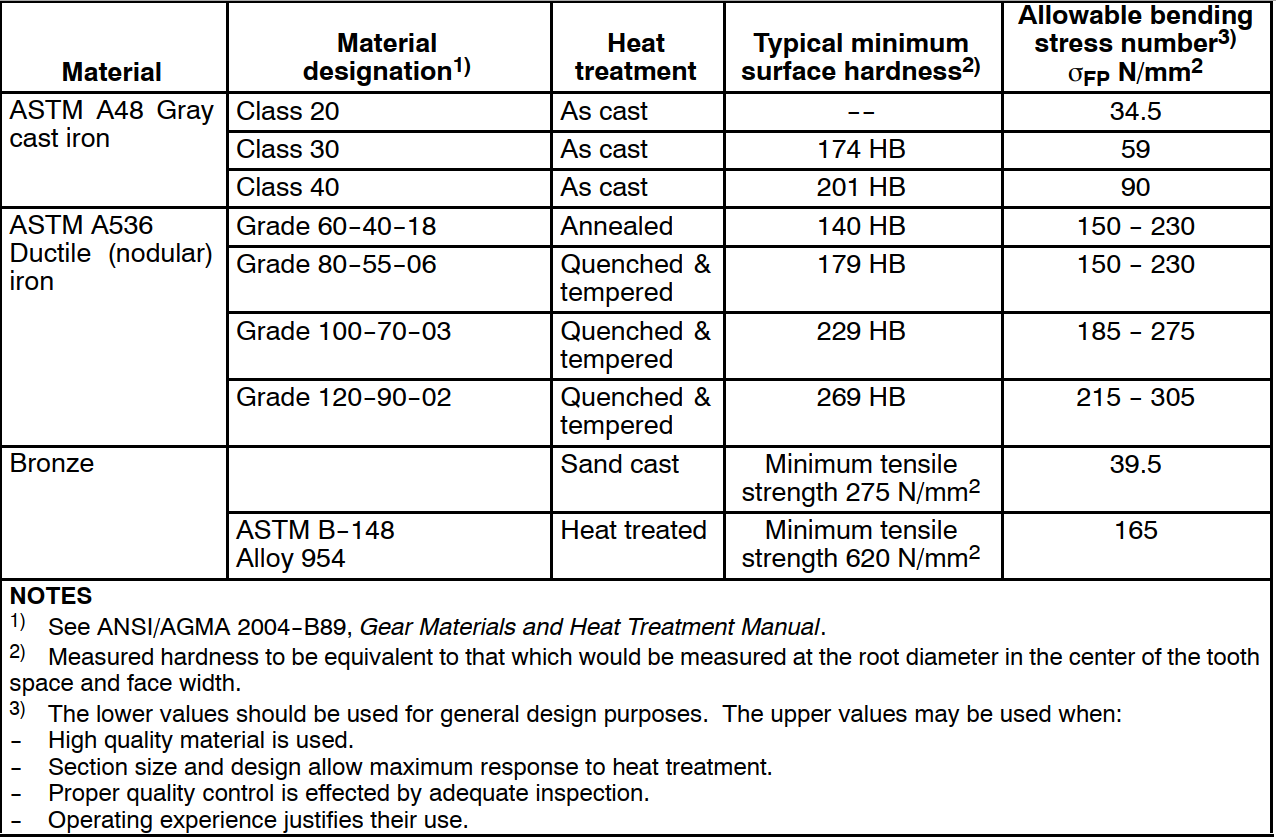
\includegraphics[scale=0.46]{Imagens/Img31.png}\\
    {\footnotesize Fonte: Adaptado de ANSI/AGMA 2101-D04 (2016)}
    \label{fig:31}
\end{figure}

Para encontrar uma dureza Brinell padronizada e seu equivalentes em
outras medidas de dureza pode ser usada a Figura
{\ref{fig:32}},~\hyperref[csl:21]{(Mott, 2013)}.\selectlanguage{brazil}

\begin{figure}[!htb]
    \centering
    \caption{Conversão de durezas}
    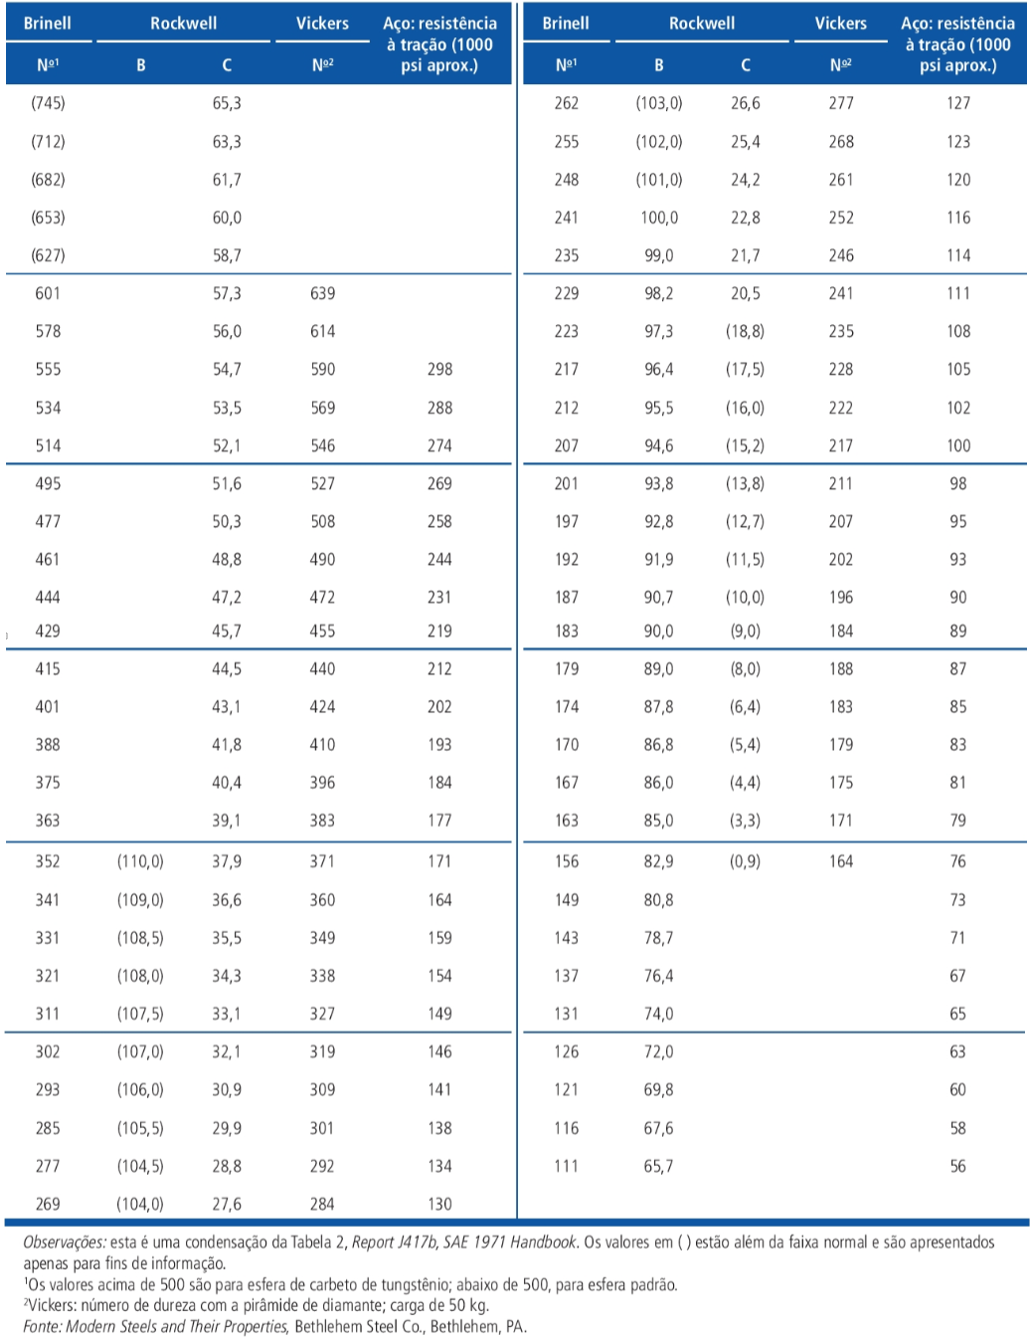
\includegraphics[scale=0.57]{Imagens/Img32.png}\\
    {\footnotesize Fonte: Adaptado de Mott (2013)}
    \label{fig:32}
\end{figure}

\section*{Aspectos Metodológicos}

{\label{aspectos-metodoluxf3gicos}}

Para a realização do presente trabalho é considerado um equipamento
real, numa indústria onde o autor trabalhou e foi possível coletar os
principais dados. Para modelar as características geométricas de uma
engrenagem , foram usadas as equações e conceitos consolidados da
literatura acadêmica da Engenharia Mecânica, especificamente na área de
Projeto de Máquinas, tais como: Elementos de Máquinas de Shigley
\hyperref[csl:20]{(Budynas \& Nisbett, 2014)}; Fundamentos do Projetos de Componentes de Máquinas
\hyperref[csl:27]{(Juvinall \& Marshek, 2011)}; e Elementos de Máquinas em Projetos Mecânicos
\hyperref[csl:21]{(Mott, 2013)}.

Para a modelagem analítica da tensão à flexão e ao contato de uma
engrenagem cilíndrica de dentes retos é usada a última versão da norma
AGMA, específicamente a direcionada para uso de unidades no sistema
internacional, ANSI/AGMA \hyperref[csl:5]{(2101-D04, 2016)}.

Para a modelagem 3D da geometria de uma engrenagem cilíndrica de dentes
retos é usada a plataforma de Projeto Assistido por Computador (CAD --
do inglês~\emph{Computer Assisted Design} ). Para a análise analítica à
flexão e ao contato é usada a plataforma de Engenharia Assistido por
Computador (CAE -- do inglês~\emph{Computer Assisted Engineering} ),
ambos na versão acadêmica do~\hyperref[csl:28]{(Solid Edge, 2020)}.

\section*{Concepção e Desenvolvimento do
Trabalho}

{\label{concepuxe7uxe3o-e-desenvolvimento-do-trabalho}}

Nesse capítulo é usado um equipamento mecânico - bomba centrífuga de
baixa velocidade -- que é acionada por um motor elétrico. No sistema de
transmissão da bomba, o pinhão está apoiado no meio de dois mancais que
estão montados na estrutura da máquina. O pinhão é cilíndrico de dentes
retos usinado e, possui um módulo de 3 mm, 16 dentes
(N\textsubscript{P}), ângulo de pressão de 20°, considera-se uma
confiabilidade de 99\%, o material usado é aço AISI 1045 Trefilado a
Frio. Além disso, considera-se:

\begin{itemize}
\tightlist
\item
  Rotação do pinhão, $\omega_P$, de 1 200 rpm;
\item
  Diâmetro do eixo de transmissão de 20 mm;
\item
  Potência no pinhão de 7 527 W;
\item
  Coroa desse sistema de transmissão de 40 dentes (N\textsubscript{G}).
\end{itemize}

Para encontrar valores relacionados às engrenagens propostas, é usada a
literatura de projeto em elemento de máquinas \hyperref[csl:20]{(Budynas \& Nisbett, 2014}; \hyperref[csl:21]{Mott, 2013}; \hyperref[csl:27]{Juvinall \& Marshek, 2011)}.

O diâmetro primitivo, \emph{D}\textsubscript{p}, do pinhão é encontrado
com a Equação {\ref{eq27}}.

\par\null

\begin{equation}
\label{eq27}
D_p=m \cdot N
\end{equation}

\par\null

Para encontrar a largura da face das engrenagens, multiplica-se o modulo
com valores de 6 a 16, a literatura recomenda multiplicar pela constante
12. Além disso, para determinar a largura da face adequada ao
engrenamento, a mesma pode ser dividida com o diâmetro primitivo e esse
produto deve ser um valor maior-igual a 0,5 e menor a 2,0.

Para encontrar a velocidade linear, \emph{V} , pode ser usada a Equação
{\ref{eq28}}.

\par\null

\begin{equation}
\label{eq28}
V=\pi \cdot D_p\cdot \omega
\end{equation}

\par\null

Conhecida a rotação do pinhão, $\omega_P$, 1 200 rpm,
para ser usada na Equação~{\ref{eq28}}, divide-se por
60, para obter 20 rps. O diâmetro primitivo considerado nessa equação
deve estar em metros.

A carga tangencial transmitida no dente do pinhão, pode ser encontrada
dividindo a potência pela velocidade linear, conforme Equação
{\ref{eq29}}.

\par\null

\begin{equation}
\label{eq29}
W^t=\frac{P}{V}
\end{equation}

\par\null

Dessa forma, substituído os valores nas equações que servem para
encontrar as características geométricas das engrenagens, obtém-se a
Tabela {\ref{tab:3}}, para o equipamento: Bomba
centrífuga de baixa rotação que é acionada por um motor elétrico .
Sempre o subscrito P, nos símbolos, significa pinhão, e o subscrito G
significa coroa.\selectlanguage{brazil}

\begin{table}[!htb]
    \centering
\caption{{\label{tab:3} Valores básicos das engrenagens}}
\begin{tabular}{l c c c c}
\hline
\multicolumn{1}{c}{\textbf{Magnitude}}  & \textbf{Simb.}   & \textbf{Valor}  & \textbf{Und.}  \\ \hline
Diâmetro do furo do cubo                & $\phi$           & 20              & mm             \\
Potência de projeto                     & P                & 7527            & W              \\
modulo                                  & m                & 3               & -              \\
Rotação de entrada                      & $\omega_P$       & 1200            & rpm            \\
Número de dentes pinhão                 & $N_P$            & 16              & -              \\
Ângulo de pressão                       & $\theta$         & 20              & $\circ$        \\
Relação de transmissão                  & i                & 2,5             & -              \\
Raio de filete                          & r                & 1,05            & mm             \\
Rotação de saída                        & $\omega_G$       & 480             & rpm            \\
Número de dentes coroa                  & $N_G$            & 40              & -              \\
Diâmetro primitivo - Pinhão             & $D_{pP}$         & 48              & mm             \\
Diâmetro externo do - Pinhão            & $D_{eP}$         & 54              & mm             \\
Diâmetro raiz - Pinhão                  & $D_{rP}$         & 40,5            & mm             \\
Diâmetro base - Pinhão                  & $D_{bP}$         & 45,1            & mm             \\
Torque do pinhão                        & $T_P$            & 59,9            & N-m            \\
Diâmetro primitivo Coroa                & $D_{pG}$         & 120             & mm             \\
Torque da coroa                         & $T_G$            & 149,74          & N-m            \\
Distância de centro                     & C                & 84              & mm             \\
Velocidade na linha primitiva           & V                & 3,016           & m/s            \\
Carga tangencial transmitida            & $W^t$            & 2495,7          & N              \\
Carga resultante transmitida            & W                & 2655,9          & N              \\
Carga radial transmitida                & $W^r$            & 908,4           & N              \\
insira largura escolhida                & b                & 36              & mm             \\ \hline
Intervalo recomendado:                  & 0,5              &$\leq b/DP<$     & 2              \\ \hline
Relação de largura da face              & b/DP             & 0,75            & -              \\ \hline
\end{tabular}
\end{table}

\subsection*{}

{\label{tensuxe3o-ao-contato-agma}}

\subsection*{Tensão ao contato AGMA}

{\label{tensuxe3o-ao-contato-agma}}

Para encontrar o coeficiente de elasticidade,~\emph{Z}\textsubscript{E},
usa-se a biblioteca~\hyperref[csl:29]{(MatWeb, 2020)} para um Aço AISI 1045, trefilado
a frio, tarugo de 50-75 mm, assim, considera-se resistência ao
escoamento de 485 Mpa, resistência à ruptura de 515 Mpa, módulo de
elasticidade 206 GPa e coeficiente de Poisson de 0,29. Neste estudo,
considera-se que ambas engrenagens são do mesmo material e mesma
largura.

Para o fator de sobrecarga considerando: fonte de alimentação motor
elétrico, uniforme e, máquina acionada: bomba centrifuga de baixa
velocidade, choque leve.

Para o fator dinâmico, considerando a velocidade linear de 3,016 m/s e o
tipo de equipamento (bomba centrífuga), o número do nível de precisão da
transmissão \emph{A}\textsubscript{V} é 10.

Para o fator de tamanho, considerando número de dentes 16. Encontra-se o
fator de forma de Lewis que é 0,296.

Para o fator de distribuição de carga, o fator de formato da face é
considerado sem coroamento no dente ou alívio na ponta do adendo.

Encontra-se o fator de proporção do pinhão, lembrando que a largura da
face é de 36 mm e o diâmetro primitivo é de 48 mm.

Para o fator de carga de deflexão, considera-se que a engrenagem está no
meio dos mancais, i.e., S\textsubscript{1}/S \textless{} 0,175.

Para o fator de alinhamento de engrenamento, consideramos a curva 1
(engrenagem aberta), visto que os mancais que a suportam estão montados
na mesma estrutura da máquina.

Para o fator de ajuste considera-se que não há nenhum ajuste na montagem
nem lapidação no dente.

Conforme a literatura científica, considera-se que a engrenagem mais
crítica é o pinhão. Sendo assim, analisa-se a tensão ao contato AGMA do
pinhão, obtendo-se os valores da Tabela~{\ref{tab:4}}.\selectlanguage{brazil}

\begin{table}[!htb]
    \centering
    \caption{{\label{tab:4} Valores de tensão ao contato AGMA no pinhão}}
    \begin{tabular}{l c c c}
\multicolumn{1}{c}{\textbf{Magnitude}}                                                                                       & \textbf{Simb.} & \textbf{Valor} & \textbf{Und.} \\ \hline
Módulo de elasticidade                                                                                                       & $E_P$             & 206000         & MPa           \\
Proporção de Poisson                                                                                                         & $v_P$             & 0,29           & -             \\
Módulo de elasticidade                                                                                                       & $E_G$             & 206000         & MPa           \\
Proporção de Poisson                                                                                                         & $v_G$             & 0,29           & -             \\
Calcular coeficiente elástico                                                                                                & $Z_E$             & 189,2          & -             \\
Insira Fator de sobrecarga                                                                                                   & $k_O$             & 1,25           & -             \\
Insira: índice de qualidade                                                                                                  & $A_v$             & 10             & -             \\
Constantes para calcular Fator dinâmico                                                                                      & B              & 0,731          & -             \\
Constantes para calcular Fator dinâmico                                                                                      & C              & 4,637          & -             \\
Fator dinâmico                                                                                                               & $k_V$             & 1,26           & -             \\
Insira fator de forma                                                                                                        & Y              & 0,296          & -             \\
Fator de tamanho                                                                                                             & $k_S$             & 1,05           & -             \\
Insira formato da face do dente                                                                                              & $K_{Hmc}$           & 1,0              & -             \\
Insira ajustes de montagem                                                                                                   & $K_{He}$            & 1,0              & -             \\
Insira carga de flexão                                                                                                       & $K_{pm}$            & 1,0              & -             \\
Se 25 $< d <$ 432                                                                                                           & $K_{Hpf}$           & 0,055          & -             \\
\multirow{3}{*}{\begin{tabular}[c]{@{}l@{}}Constantes para fator de alinhamento.\\ Mancais montados na máquina \\ -
\end{tabular}}

& A              & 0,247          & -             \\
                                                                                                                             & B              & 0,000657       & -             \\
                                                                                                                             & C              & -1,186E-07     & -             \\
                                                                                             
Fator de alinhamento                                                                                                         & $K_{Hma}$           & 0,27           & -             \\
Fator de distribuição de carga                                                                                               & $k_H$             & 1,33           & -             \\
Inserir Fator de condição de superficial                                                                                     & $Z_R$             & 1,0              & -             \\
Seno de ângulo de pressão 20                                                                                                 & sen$\theta$           & 0,342          & -             \\
Cosseno de ângulo de pressão 20                                                                                              & cos$\theta$           & 0,940          & -             \\
Fator de curvatura na linha primitiva                                                                                        & $C_c$             & 0,115          & -             \\
Fator para ajuste da altura específica 1                                                                                     & $C_1$             & 2,736          & -             \\
Fator para ajuste da altura específica 2                                                                                     & $C_2$             & 6,840          & -             \\
Fator para ajuste da altura específica 3                                                                                     & $C_3$             & 2,952          & -             \\
Fator para ajuste da altura específica 4                                                                                     & $C_4$             & 2,212          & -             \\
Fator para ajuste da altura específica do LPSTC                                                                              & $C_x$             & 0,809          & -             \\
Calcular Fator geométrico de crateramento                                                                                    & $Z_I$             & 0,093          & -             \\
Tensão de Contato AGMA                                                                                                       & $\sigma_H$              & 1106,36        & MPa             \\ \hline  
\end{tabular}
\end{table}

\subsection*{}

{\label{fator-de-seguranuxe7a-ao-contato-agma}}

\subsection*{Fator de segurança ao contato
AGMA}

{\label{fator-de-seguranuxe7a-ao-contato-agma}}

Primeiramente, encontra-se o fator de ciclagem de tensão ao contato.
Para encontrar o número de ciclos de tensão, considera-se a vida nominal
como a de um equipamento industrial a 30 000 horas de trabalho, também
considera-se apenas um sentido de giro da engrenagem.

Para o fator de temperatura, considera-se que a engrenagem não
trabalhará a temperaturas superiores a 120 °C.

Sabe-se que uma engrenagem que opera na indústria deve ter uma dureza na
superfície do dente, como a dureza não foi indicada, a seguir, deve-se
encontrar a dureza adequada para a engrenagem de aço. Assim, o fator de
segurança ao contato AGMA, deve estar no intervalo de 1 a 1,5. Para este
estudo considera-se inicialmente o~\emph{S}\textsubscript{H} 1,0 com o
objetivo de encontrar uma dureza Brinell (HB) estimada.

Dessa forma, inicialmente obtém-se um número de tensão ao contato
permitido de 1251,93 MPa. Assim, pode ser encontrada a dureza HB próxima
à desejada. Para tal, considerando grau 1, da Figura
{\ref{fig:21}}, para uma engrenagem fabricada de aço.

Ajustando a dureza HB obtida, a um padrão comercial, mas, que seja logo
a próxima superior à encontrada, usando a Figura
{\ref{fig:32}} ajusta-se a dureza inicial de 473,8 para
477 HB.

Assim, na Tabela~{\ref{tab:5}}, encontram-se os valores
considerados para calcular o fator de segurança ao contato, que é também
1,0, equivalente ao valor inicialmente assumido para determinar a dureza
a ser solicitada, para a engrenagem que está sendo projetada.\selectlanguage{brazil}

\begin{table}[!htb]
\centering
\caption{{\label{tab:5} Valores obtidos para o fator de segurança ao contato AGMA}}
\begin{tabular}{l c c c c}
\hline
\multicolumn{1}{c}{\textbf{Magnitude}}    & \textbf{Simb.} & \textbf{Valor} & \textbf{Und.} \\ \hline
Insira vida em horas                      & L              & 30000          & h             \\
Insira revolução                          & $\omega_P$              & 1200           & rpm           \\
Insira número de contatos/revolução       & q              & 1,0              & -             \\
Número de ciclos de tensão                & $n_L$             & 2,16E+9        & -             \\
Fator de ciclagem de tensão               & $Z_N$             & 0,884          & -             \\
Fator de razão de dureza Pinhão           & $Z_W$             & 1,0              & -             \\
Inserir Fator de temperatura              & $Y_\theta$              & 1,0              & -             \\
Inserir Fator de confiabilidade           & $Y_Z$              & 1,0              & -             \\
Inserir Fator de segurança HIPÓTESE       & $S_H$             & 1,0              & -             \\
Número ao contato permitido Preliminar    & $\sigma_{HP}$             & 1251,93        & -             \\
Dureza Brinell grau 1 para Aço Preliminar & HB             & 473,84         & -             \\
Inserir HB escolhido ver Figura 29        & HB             & 477            & -             \\
Número ao contato permitido Final         & $\sigma_{HP}$             & 1258,94        & MPa           \\
Fator de segurança RECALCULADO            & $S_H$             & 1,0            & -    \\ \hline        
\end{tabular}
\end{table}

\subsection*{}

{\label{tensuxe3o-uxe0-flexuxe3o-agma}}

\subsection*{Tensão à flexão AGMA}

{\label{tensuxe3o-uxe0-flexuxe3o-agma}}

Para encontrar a tensão à flexão, muitos dos fatores já foram
encontrados anteriormente e algum deles podem ser encontrados na
Tabela~{\ref{tab:4}}.

Para encontrar o fator de espessura de borda, primeiro encontra-se a
altura do dente da engrenagem, considerando um dente de profundidade
completa e ângulo de pressão 20°, usa-se a Equação
{\ref{eq30}}, \hyperref[csl:20]{(Budynas \& Nisbett, 2014)}:

\par\null

\begin{equation}
\label{eq30}
h_t = m+1,25 \cdot m
\end{equation}



Considera-se, também, que o furo da engrenagem de 20 mm (diâmetro do
eixo onde será montada a engrenagem), apresenta um~ canal de chaveta no
cubo, seguindo a norma DIN~\hyperref[csl:30]{(6885 A, 1968)}, de
t\textsubscript{R}=7,45. Assim:

\begin{equation}
m_{B}=\frac{7,45}{6,75}=1,104<1,2 \nonumber \\
\end{equation}

Para o fator geométrico da resistência à flexão, 
considera-se número de dentes do pinhão de 16 (eixo x da
Figura~{\ref{fig:25}}) e número de dentes da coroa de
40 (eixo y da Figura~{\ref{fig:25}}), obtendo o valor
de 0,27.

Finalmente, na Tabela {\ref{tab:6}}, apresenta-se os
valores usados para encontrar a tensão à flexão AGMA, no dente do
pinhão.\selectlanguage{brazil}

\begin{table}[!htb]
\centering
\caption{{\label{tab:6} Valores obtidos para a tensão à flexão}}
\begin{tabular}{l c c c c}
\hline
\multicolumn{1}{c}{\textbf{Magnitude}}           & \textbf{Simb.} & \textbf{Valor} & \textbf{Und.} \\ \hline
Insira altura do dente                           & $h_t$             & 6,75           & mm            \\
Insira altura da borda                           & $t_R$             & 7,1            & mm            \\
relação de alturas                               & $m_B$             & 1,052          & -             \\
Se $m_B < 1,2$ \ então\ o\ fator\ de\ espessura\ de\ borda & $k_B$             & 1,211          & -             \\
Inserir Fator geométrico de flexão, (Pinhão)      & $Y_J$             & 0,27           & -             \\
Tensão de Flexão AGMA                            & $\sigma_F$       & 227,71         & MPa     \\ \hline    
\end{tabular}
\end{table}

\subsection*{}

{\label{fator-de-seguranuxe7a-uxe0-flexuxe3o-agma}}

\subsection*{Fator de segurança à flexão
AGMA}

{\label{fator-de-seguranuxe7a-uxe0-flexuxe3o-agma}}

Nesta seção, muitos dos fatores para o fator de segurança, já foram
encontradas anteriormente. Para o fator de ciclagem para resistência à
flexão, considera-se que o número de ciclos permitido é levando em
consideração, também, 30 000 h de trabalho.

Os fatores de confiabilidade e temperatura são os mesmos já encontrados
anteriormente. Além disso, como já foi determinada a dureza para a
tensão ao contato, a mesma dureza também deve ser considerado para o
cálculo da tensão à flexão, ou seja, 477 HB.

Dessa forma, na Tabela {\ref{tab:7}} são apresentados
os valores considerados para o fator de segurança à flexão AGMA no dente
do pinhão.\selectlanguage{brazil}

\begin{table}[!htb]
\centering
\caption{{\label{tab:7} Valores para o fator de segurança à flexão AGMA}}
\begin{tabular}{l c c c c}
\hline
\multicolumn{1}{c}{\textbf{Magnitude}}       & \textbf{Simb.}  & \textbf{Valor} & \textbf{Und.} \\ \hline
Fator de ciclagem de tensão                  & $Y_N$             & 0,925          & -            \\
Inserir HB escolhido                         & HB              & 477            & -            \\
Número à flexional permitido RECALCULADO     & $\sigma_{FP}$    & 342,5          & MPa             \\
Fator de segurança RECALCULADO               & $S_F$              & 1,4            & -             \\ \hline     
\end{tabular}
\end{table}

\subsection*{}

{\label{anuxe1lise-de-tensuxe3o-uxe0-flexuxe3o-e-ao-contato-computacional}}

\subsection*{Análise de Tensão à flexão e ao contato
computacional}

{\label{anuxe1lise-de-tensuxe3o-uxe0-flexuxe3o-e-ao-contato-computacional}}

Uma forma de validar os resultados oriundos de modelos analíticos é por
meio de FEM. Conforme o levantamento do estado da arte, (Introdução),
para uma FEA pode ser considerado apenas 3 dentes de um pinhão no ponto
mais crítico, ou seja, no pinhão em estudo é onde o dente do pinhão
coincide com o canal de chaveta do cubo.

Neste trabalho não é usado o software ANSYS, mas, pretende-se fazer isso
num futuro trabalho. Considera-se o software Solid Edge para uma análise
estática que permita verificar o efeito da aplicação de apenas a carga
tangencial ou ambas as cargas (tangencia e radial), no dente de uma
engrenagem. Para tal, é usado na representação da geometria do pinhão, o
software Solid Edge versão acadêmica, especificamente a plataforma CAD.

Ainda, na informação colhida no estado da arte, uma das vantagens da
norma AGMA é que usa ambas cargas para análise, concentradas no diâmetro
primitivo do dente de uma engrenagem, já a norma ISO considera apenas a
carga tangencial.

De acordo à literatura, podemos encontrar, a partir da carga tangencial
e o ângulo de pressão, a carga resultante (tangencial e radial)
\hyperref[csl:20]{(Budynas \& Nisbett, 2014}; \hyperref[csl:21]{Mott, 2013}; \hyperref[csl:27]{Juvinall \& Marshek, 2011)}.

Assim, na Figura {\ref{fig:33}} observa-se que quando
considerada apenas a carga tangencial , neste caso de 2495,7 N, para o
teste estático de simulação com uma malha de 1,68 mm de afastamento
entre seus pontos, apresenta no ponto do diâmetro primitivo, a 1 mm
aproximadamente de profundidade, uma tensão de 65 MPa. E na superfície
do cordão raiz a tensão apresentada é também de aproximadamente 65 MPa.\selectlanguage{brazil}

\begin{figure}[!htb]
    \centering
    \caption{FEA considerando apenas carga tangencial}
    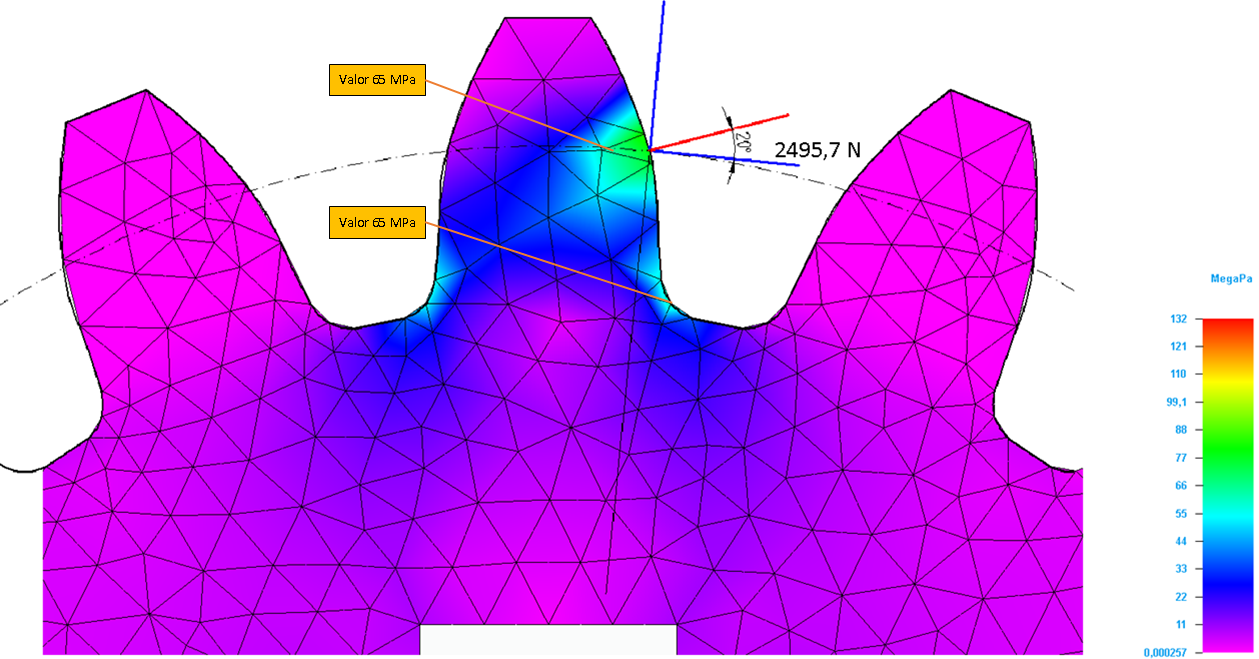
\includegraphics[scale=0.46]{Imagens/Img33.png}\\
    {\footnotesize Fonte: Adaptado  Autoria própria}
    \label{fig:33}
\end{figure}

Por outro lado, na Figura {\ref{fig:34}} observa-se que
são consideradas ambas cargas (tangencial e radial), contidas na carga
resultante de 2 655,9 N. Nesse segundo estudo estático de simulação
considerou-se também uma malha de 1,68 mm de afastamento entre seus
pontos. Percebe-se que no ponto do diâmetro primitivo, também a 1 mm
aproximadamente de profundidade, a tensão apresentada é de 65 MPa. E na
superfície do cordão raiz a tensão a tração apresentada é de
aproximadamente 52 MPa, e uma tensão de compressão de aproximadamente 60
MPa.\selectlanguage{brazil}

\begin{figure}[!htb]
    \centering
    \caption{FEA considerando carga resultante}
    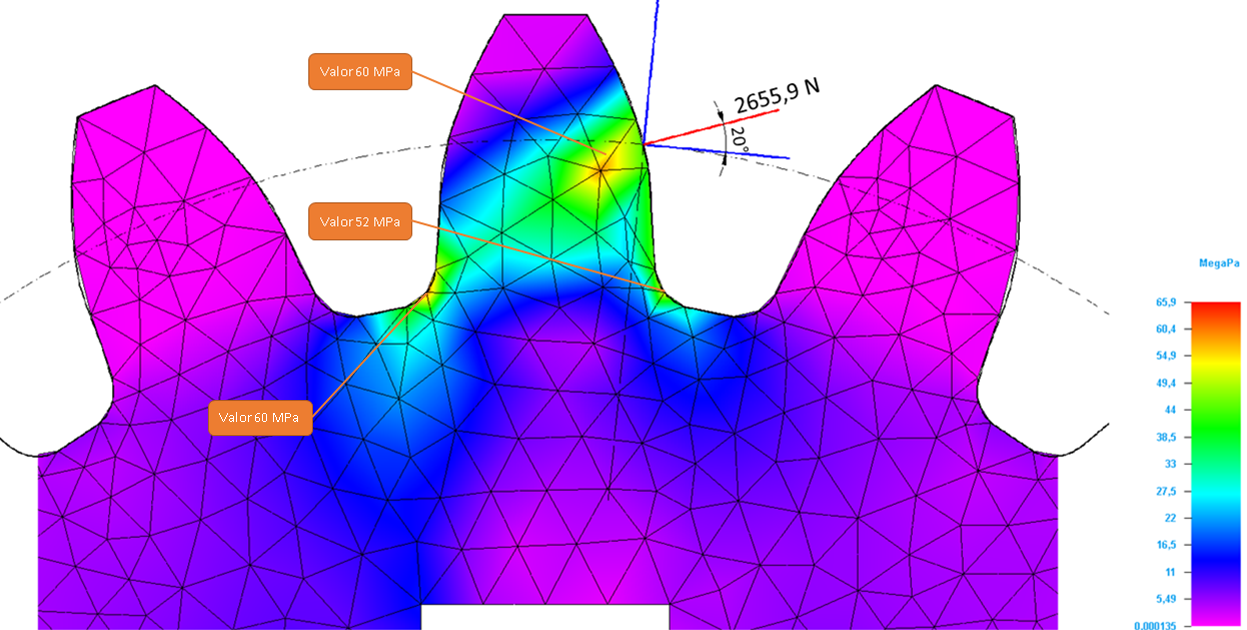
\includegraphics[scale=0.46]{Imagens/Img34.png}\\
    {\footnotesize Fonte: Adaptado  Autoria própria}
    \label{fig:34}
\end{figure}

Ambos testes, Figuras {\ref{fig:33}} e
{\ref{fig:34}}, tiveram as mesmas condições de entrada,
mas, claramente o estudo com apenas a carga tangencial aplicada, embora
inferior quando comparada com a carga resultante, apresenta pontos com
tensões mais elevadas, fato que confirma que quando é considerada apenas
a carga tangencial numa modelagem analítica de cálculo de tensão, a
mesma deve ser mais conservadora. Também, pode ser comprovado que a
carga radial ajuda a mitigar as tensões no dente da engrenagem.

A continuação, os cálculos para o pinhão em análise que usa a norma AGMA
2101-D04 (2016) e a literatura de acadêmica \hyperref[csl:20]{(Budynas \& Nisbett, 2014}; \hyperref[csl:21]{Mott, 2013}; \hyperref[csl:27]{Juvinall \& Marshek, 2011)}, é
denominado de~\textbf{Estudo1}. Já os cálculos obtidos do programa Solid
Edge, especificamente usando a plataforma CAE, para uma análise à fadiga
é denominado de~\textbf{Estudo2}. Segundo o fabricante do software Solid
Edge, o mesmo considera para esse tipo de cálculo a norma ISO 6336.

Na Tabela \ref{tab:8} é apresentado um comparativo entre o estudo 1 e 2. A
maioria dos valores para a construção da geometria do pinhão e outros
valores básicos, são iguais em ambos estudos, a maior diferença é na
construção da involuta do dente, o~\textbf{Estudo1} considera o critério
de Lewis, e o \textbf{Estudo2} considera o critério da norma ISO.\selectlanguage{brazil}

\begin{table}[!htb]
\centering
\caption{{\label{tab:8} Resultados para o fator de segurança à flexão AGMA}}
\begin{tabular}{l c c c c}
\hline
\multicolumn{1}{c}{\textbf{Magnitude}} & \textbf{Estudo1} & \textbf{Estudo2} \\ \hline
Diâmetro externo              & 54 mm       & 54 mm         \\
Diâmetro primitivo            & 48 mm       & 48 mm         \\
Diâmetro base                 & 45,1 mm     & 45,1 mm       \\
Diâmetro raiz                 & 40,5 mm     & 40,5 mm       \\
Distância de centro           & 84 mm       & 84 mm         \\
Involuta                      & Lewis       & ISO           \\
Relação de largura da face    & 0,75        & 0,75          \\
Velocidade linear             & 3,016 m/s   & 3,016 m/s     \\
Carga tangencial              & 2495,7 N    & 2495,75       \\
Carga radial                  & 908,4 N     & 908,38        \\
Carga resultante              & 2655,9 N    & 2655,9        \\
Torque do pinhão              & 59,897 N-m  & 58,898 N-m    \\ \hline
\end{tabular}
\end{table}

Na Tabela {\ref{tab:9}} são apresentados os principais
fatores considerados para cálculo de tensão à flexão e ao contato na
norma AGMA e o seu equivalente no software Solid Edge. O fator de
sobrecarga no Solid Edge é chamado de fator de aplicação e ambos são
iguais. O fator de distribuição de carga no Solid Edge é chamado de
fator de montagem, sendo diferentes, mesmo considerando critérios iguais
na entrada de dados. O fator dinâmico possui o mesmo nome, mas, os
valores são diferentes. No programa Solid Edge solicita-se a alimentação
de um fator de aspereza que não existe na norma AGMA, podendo supor que
seja parte do fator dinâmico, mas não há informação suficiente para
poder afirmar isso. O fator de tamanho possui o mesmo nome e seus
valores são muito próximos. O coeficiente de elasticidade é chamado no
Solid Edge de fator de elasticidade e ambos são muito próximos.
Finalmente, para que a comparação seja mais consistente, e como já foram
encontrados os valores para o número de tensão permitido, tanto para
flexão e contato, esses valores são alimentados, como dados de entrada,
no Solid Edge.\selectlanguage{brazil}

\begin{table}[!htb]
\centering
\caption{{\label{tab:9} Fatores considerados em ambos estudos}}
\begin{tabular}{l c c c c}
\hline
\multicolumn{1}{c}{\textbf{Magnitude}} & \textbf{Estudo1} & \textbf{Estudo2} \\ \hline
Fator de sobrecarga                 & 1,25              & 1,25 \\
Fator de distribuição de carga      & 1,33              & -0,08 \\
Fator dinâmico                      & 1,26              & 1,01  \\
Fator de aspereza                      & -                 & 1,15              \\
Fator de tamanho                       & 1,05              & 1,00              \\
Fator de elasticidade                  & 189,19            & 189,81            \\
Número de flexão permitido             & 342,541 MPa       & 342,541 MPa       \\
Número de contato permitido            & 1258,94 MPa       & 1258,94 MPa   \\ \hline  
\end{tabular}
\end{table}

Finalmente, na Figura~{\ref{fig:35}} são apresentados e
comparados os resultados já calculados usando a norma AGMA e os obtidos
no programa Solid Edge. Conclui-se que a tensão à flexão é o único valor
que no software Solid Edge é inferior, 25,05\% menor, mas, o fator de
segurança à flexão no Solid Edge é 48,15\% superior. A tensão ao contato
é superior no Solid Edge em 16,77\% e o fator de segurança no Solid Edge
é 42,2\% superior em relação à norma AGMA.\selectlanguage{brazil}

\begin{figure}[!htb]
    \centering
    \caption{Tensões e fatores de segurança para flexão e contato}
    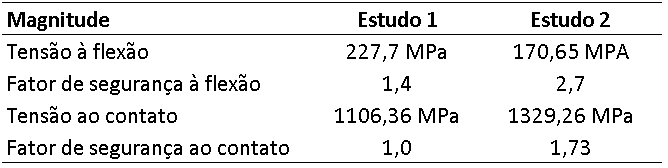
\includegraphics[scale=0.65]{Imagens/Img35.png}\\
    {\footnotesize Fonte: Autoria própria}
    \label{fig:35}
\end{figure}



\section*{Conclusão}

{\label{conclusuxe3o}}

Neste trabalho foi realizado o estado da arte do cálculo à fadiga em
engrenagens cilíndricas, destacando 4 formas na literatura cientifica:
i) testes experimentais, mas, um dos pontos negativos é o custo para
fabricar protótipos físicos para ensaios, além de que os mesmos têm que
ser reproduzidos numa escala superior ao elemento real, para minimizar
os erros no posicionamento de sensores e consequente coleta de dados;
ii) análise computacional, principalmente destacam-se o ANSYS e ABAQUS,
mas os mesmos apresentam pontos negativos em relação a custos com
processadores computacionais para obter resultados preciso e rápidos,
custo para aquisição do software, além disso, embora tenham ocorrido
muitas melhorias nas suas versões para a modelagem 3D de um elemento,
ainda não são tão amigáveis quando comparado a outros programas
específicos de CAD, tais como o Solid Edge; iii) modelagem analítica
usando a norma ISO 6336, mas, um dos pontos negativos é que dita norma
considera apenas a carga tangencial nos seus cálculos, fato que obriga à
mesma ser bem conservadora nos seus resultados, outro inconveniente é
não estar difundida no mundo acadêmico a sua nova versão de 2019, além
de apresentar um custo relativamente alto para sua aquisição; iv)
modelagem analítica usando a norma ANSI/AGMA~\hyperref[csl:5]{(2101-D04, 2016)} para o
Sistema Internacional, apresenta-se como a mais rápida e fácil de ser
usada para cálculos à fadiga de tensão à flexão e ao contato, além de
ser mais divulgada nas pesquisas científicas, considera nos seus
cálculos as cargas tangencial e radial, possibilidade de aquisição da
norma a um valor mais baixo para fins acadêmicos, e mesmo se adquirida
comercialmente, a mesma é 60\% mais barata do que a norma ISO. Um ponto
negativo da norma AGMA é que não considera, ainda, nos seus cálculos um
fator para avaliar o impacto no adendo da ponta do dente de uma
engrenagem, fenômeno que diminui a tensão à flexão e ao contato, além de
deixar o engrenamento mais suave.

Destaca-se também neste trabalho que a aparição de uma possível fratura
ao contato apresenta-se depois de 10\textsuperscript{7} ciclos a mais de
1 mm de profundidade em relação à superfície do flanco do dente de
engrenagem, considerando que a engrenagem possui algum tipo de
tratamento térmico na sua superfície. Outro dado importante que pode
minimizar o tempo de processamento para uma FEA é a confirmação de que
analisando apenas a geometria de 3 dentes de uma engrenagem,
independentemente do número total de dentes, podem ser obtidos
resultados confiáveis. Também, o estado da arte aponta que um alívio no
adendo da ponta do dente de uma engrenagem, (acima do diâmetro
primitivo), proporciona um engrenamento mais leve e diminui a tensão de
contato com o dedendo, (abaixo do diâmetro primitivo), do dente que
engrena, mas, se esse alívio não for calculado pode influenciar
negativamente no aumento da tensão à flexão. Além disso, normalmente na
literatura acadêmica considera-se que o cordão raiz é o produto do
módulo vezes a constante de 0,3 ou 0,35, já nos estudos recentes são
usados para o cordão raiz, a multiplicação do módulo pela constante
0,38, dessa forma há maior dissipação da tensão no filete do dente .

Outro aporte deste trabalho é o detalhamento da norma AGMA 2101-D04 e a
inclusão de tabelas e gráficos da literatura acadêmica, proporcionando
assim, um protocolo para seu uso e modelagem analítica de qualquer tipo
de engrenagem cilíndrica de dentes retos. Além disso é disponibilizada
uma
\href{https://docs.google.com/spreadsheets/d/19pnUCaySImdiL_x95e3OEQRMFw082qtCaUppl3dgY9c/edit?usp=sharing}{planilha}
com todos os equacionamentos, fácil de ser descarregada. Isto
possibilitará que em futuros trabalhos possa ser desenvolvido dito
equacionamento em códigos de linguagem de programação como o Python,
fortalecendo uma das vulnerabilidades que possui o uso de uma planilha
Excel, por exemplo.

No item concepção e desenvolvimento deste trabalho, foram usados dados
reais de um equipamento conhecido pelo autor. Foi modelada a forma
analítica da engrenagem usando a norma AGMA 2101-D04 (2016) e
comparou-se com resultados obtidos no software Solid Edge que na sua
biblioteca indica usar a norma ISO 6336. Comprovou-se que há divergência
nos resultados obtidos e de uma forma geral os resultados do Solid Edge
são mais conservadores que a norma AGMA, mesmo cenário relatado no
estado da arte quando comparadas as normas AGMA e ISO.

Finalmente, pretende-se em futuros trabalhos automatizar a norma AGMA
2101-D04 criando códigos de programação no Python. Além disso,
pretende-se com a publicação deste trabalho, convidar outros
pesquisadores para analisar os dados deste trabalho no software ANSYS ou
ABAQUS.

\selectlanguage{brazil}
\FloatBarrier
\section*{\refname}\sloppy
\phantomsection
\label{csl:1}Learning, C. (Ed.). (2015). \textit{{Introdução à Engenharia Mecânica}} (2nd ed.). Cengage Learning.

\phantomsection
\label{csl:2}{Equipamentos mecânicos: Análise de falhas e solução de problemas}. (2012). In QualityMark (Ed.), \textit{Rio de Janeiro: Editora Qualitymark} (3rd ed.).

\phantomsection
\label{csl:3}{External spur gear root bending stress: A comparison of ISO 6336:2006, AGMA 2101-D04, ANSYS finite element analysis and strain gauge techniques}. (2017). \textit{Mechanism and Machine Theory}, \textit{111}, 1–9. \url{https://doi.org/10.1016/j.mechmachtheory.2017.01.006}

\phantomsection
\label{csl:4}\textit{{Dynamic structural and thermal characteristics analysis of oil-lubricated multi-speed transmission gearbox: variation of load, rotational speed and convection heat transfer}}. (2006). International Organization for Standardization. \url{https://www.iso.org/standard/63822.html}

\phantomsection
\label{csl:5}\textit{{Fundamental rating factors and calculation methods for involute spur and helical gears teeth}}. (2016). American Gear Manufacturers Association. \url{https://members.agma.org/ItemDetail?iProductCode=2101-D04\&Category=STANDARDS}

\phantomsection
\label{csl:6}{Analytical load sharing and mesh stiffness model for spur/helical and internal/external gears – Towards constant mesh stiffness gear design}. (2017). \textit{Mechanism and Machine Theory}, \textit{113}, 126–140. \url{https://doi.org/10.1016/J.MECHMACHTHEORY.2017.03.007}

\phantomsection
\label{csl:7}{A new analytical model to calculate the maximum tooth root stress and critical section location of spur gear}. (2018). \textit{Mechanism and Machine Theory}, \textit{128}, 275–286. \url{https://doi.org/10.1016/J.MECHMACHTHEORY.2018.05.012}

\phantomsection
\label{csl:8}{Modeling of contact fatigue damage behavior of a wind turbine carburized gear considering its mechanical properties and microstructure gradients}. (2019). \textit{International Journal of Mechanical Sciences}, \textit{156}, 283–296. \url{https://doi.org/10.1016/J.IJMECSCI.2019.04.004}

\phantomsection
\label{csl:9}{An analytical method for calculating the tooth surface contact stress of spur gears with tip relief}. (2019). \textit{International Journal of Mechanical Sciences}, \textit{151}, 170–180. \url{https://doi.org/10.1016/J.IJMECSCI.2018.11.007}

\phantomsection
\label{csl:10}\textit{{Calculation of load capacity of spur and helical gears: Calculation of surface durability (pitting)}}. (2006). International Organization for Standardization. \url{https://www.iso.org/standard/63821.html}

\phantomsection
\label{csl:11}{A quasi-static FEM for estimating gear load capacity}. (2015). \textit{Measurement}, \textit{75}, 40–49. \url{https://doi.org/10.1016/J.MEASUREMENT.2015.07.036}

\phantomsection
\label{csl:12}{Analysis and formulation of spur gear stresses with different tip modifications}. (2019). \textit{Journal of Central South University}, \textit{26}(9), 2368–2378. \url{https://doi.org/10.1007/s11771-019-4180-x}

\phantomsection
\label{csl:13}{A New Experimental Approach to Test Open Gears for Winch Drums}. (2015). \textit{Procedia Engineering}, \textit{133}, 192–201. \url{https://doi.org/10.1016/J.PROENG.2015.12.657}

\phantomsection
\label{csl:14}{Contact stress analysis for a pair of mating gears}. (2013). \textit{Mathematical and Computer Modelling}, \textit{57}(1–2), 40–49. \url{https://doi.org/10.1016/J.MCM.2011.06.055}

\phantomsection
\label{csl:15}{A translation technique: Dimensionless ratings and conversion factors between ISO and AGMA gear standards}. (2016). \textit{ASME International Mechanical Engineering Congress and Exposition, Proceedings (IMECE)}, \textit{11}. \url{https://doi.org/10.1115/IMECE201665123}

\phantomsection
\label{csl:16}{Dynamic structural and thermal characteristics analysis of oil-lubricated multi-speed transmission gearbox: variation of load, rotational speed and convection heat transfer}. (2017). \textit{Iranian Journal of Science and Technology, Transactions of Mechanical Engineering}, \textit{41}(4), 281–291. \url{https://link.springer.com/article/10.1007/s40997-016-0063-z}

\phantomsection
\label{csl:17}{Free vibration and connecting bolt constraint-based FEA analysis of heavy vehicle medium duty transmission gearbox housing made from AISI 4130 alloy material}. (2017). In \textit{Mathematics Applied to Engineering} (pp. 133–146). Elsevier. \url{https://www.sciencedirect.com/science/article/pii/B9780128109984000077}

\phantomsection
\label{csl:18}{New Siemens applications for designing bevel gears}. (2017). \textit{IOP Conference Series: Materials Science and Engineering}, \textit{227}(1), 12049. \url{https://www.researchgate.net/publication/318922770_New_Siemens_applications_for_designing_bevel_gears}

\phantomsection
\label{csl:19}{Modeling and Dynamic Simulation of TI Worm Drivebased on GearTrax}. (2019). \textit{2019 IEEE 8th Data Driven Control and Learning Systems Conference (DDCLS)}, 1355–1359. \url{https://ieeexplore.ieee.org/abstract/document/8909061}

\phantomsection
\label{csl:20}McGraw-Hill (Ed.). (2014). \textit{{Shigley’s Mechanical Engineering Design}} (10th ed.). McGraw-Hill Education.

\phantomsection
\label{csl:21}Pearson (Ed.). (2013). \textit{{Machine elements in mechanical design}} (5th ed.). Pearson.

\phantomsection
\label{csl:22}\textit{{Calculation of load capacity of spur and helical gears: Calculation of service life under variable load}}. (2006). International Organization for Standardization. \url{https://www.iso.org/standard/38788.html}

\phantomsection
\label{csl:23}\textit{{Gear Classification and Inspection Handbook - Tolerances and Measuring Methods for Unassembled Spur and Helical Gears}}. (2002). American Gear Manufacturers Association. \url{https://members.agma.org/ItemDetail?iProductCode=2000-A88\&Category=STANDARDS}

\phantomsection
\label{csl:24}{An ontology-based model for prognostics and health management of machines}. (2017). \textit{Journal of Industrial Information Integration}, \textit{6}, 33–46. \url{https://doi.org/10.1016/j.jii.2017.02.006}

\phantomsection
\label{csl:25}{{OntoProg}: An ontology-based model for implementing Prognostics Health Management in mechanical machines}. (2018). \textit{Advanced Engineering Informatics}, \textit{38}, 746–759. \url{https://doi.org/10.1016/j.aei.2018.10.006}

\phantomsection
\label{csl:26}{Determination of the bending strength geometry factor J for the calculation of stress in parallel-axis gears as a function of the reference correction and slope angle of the gear tooth}. (2016). \textit{Int. J. Mech. Eng. Autom}, \textit{3}(1), 27–33. \url{https://pdfs.semanticscholar.org/2b6c/c698e8d5e5a35c59e68094c409da395b9d1c.pdf}

\phantomsection
\label{csl:27}Sons, J. W. \& (Ed.). (2011). \textit{{Fundamentals of machine component design}} (5th ed.). John Wiley \& Sons.

\phantomsection
\label{csl:28}\textit{{Solid Edge for Educators}}. (2020). Siemens PLM Software. \url{https://www.plm.automation.siemens.com/global/pt/our-story/partners/academic/engineering-curriculum.html}

\phantomsection
\label{csl:29}\textit{{Source for Materials Information}}. (2020). MatWeb Materail Property Data. \url{http://www.matweb.com/}

\phantomsection
\label{csl:30}\textit{{Drive Type Fastenings without Taper Action; Parallel Keys, Keyways, Deep Pattern}}. (1968). Deutsches Institut für Normung. \url{https://www.din.de/en/getting-involved/standards-committees/nam/standards/wdc-beuth:din21:506020}
\end{document}